\let\texyear\year % ieeeaccess.cls redefines \year, which breaks TikZ (quantikz)
\documentclass{ieeeaccess}
\usepackage{cite}
\usepackage{amsmath,amssymb,amsfonts}
\usepackage{algorithmic}
\usepackage{algorithm}
\usepackage{graphicx}
\graphicspath{{imgs/}}
\usepackage{textcomp}
\usepackage{booktabs}
\usepackage{float} % [H] placement: float stays exactly where it is in the source
\usepackage{physics}
\usepackage{multirow}
\let\accessyear\year \let\year\texyear
\usepackage{quantikz}
\let\year\accessyear
\definecolor{accessblue}{cmyk}{1,0.3,0,0.2} % class defines it as a spot color, which xcolor (loaded by TikZ) can't use
\definecolor{greycolor}{cmyk}{0,0,0,.8}
\def\xfigwd{0pt} % class captions expect \xfigwd, normally set only by its \Figure macro
\def\headerlogo{}\def\headerlogoall{} % university draft: no journal logo in the header
% university draft: footer shows only the page number, title block drops the history/DOI lines
\usepackage{etoolbox}
\makeatletter
\let\accessps@headings\ps@headings
\def\ps@headings{\accessps@headings
  \def\@oddfoot{\hfill\raisebox{8pt}{\footerpagefont\thepage}}%
  \def\@evenfoot{\raisebox{8pt}{\footerpagefont\thepage}\hfill}}
\let\accessps@titlepage\ps@titlepage
\def\ps@titlepage{\accessps@titlepage
  \def\@oddhead{}\def\@evenhead{}%
  \def\@oddfoot{\hfill\raisebox{3pt}{\footerpagefont\thepage}}%
  \def\@evenfoot{\raisebox{3pt}{\footerpagefont\thepage}\hfill}}
\pagestyle{headings}
\patchcmd{\@maketitle}{{\vss\historyfont\@history\vss}\vspace*{2mm}\par}{}{}{}
\patchcmd{\@maketitle}{{\vss\doifont Digital Object Identifier\space\@doi\vss}\vspace*{7.4mm}\par}{}{}{}
\makeatother

\newtheorem{definition}{Definition}[section]
\newtheorem{theorem}{Theorem}[section]
\newtheorem{proposition}{Proposition}[section]
\newtheorem{corollary}{Corollary}[section]
\newtheorem{lemma}{Lemma}[section]

\def\BibTeX{{\rm B\kern-.05em{\sc i\kern-.025em b}\kern-.08em
    T\kern-.1667em\lower.7ex\hbox{E}\kern-.125emX}}
\begin{document}
\history{Date of publication xxxx 00, 0000, date of current version xxxx 00, 0000.}
\doi{10.1109/TQE.2020.DOI}

\title{A study of experimental privacy budget quantification in quantum differential privacy simulations}
\author{\uppercase{Tomas Sierra Sanchez}\authorrefmark{1},
\uppercase{Valérie E. Gauthier-Umaña\authorrefmark{2}, and Juan F. Perez}.\authorrefmark{3}}
\address[1]{Department of Systems and Computing Engineering, Universidad de los Andes  (email: t.sierras@uniandes.edu.co)}
\address[2]{Advisor, Department of Systems and Computing Engineering, Universidad de los Andes, Bogotá D.C, Colombia}
\address[3]{Advisor, Department of Industrial Engineering, Universidad de los Andes, Bogotá D.C, Colombia (email: jf.perez33@uniandes.edu.co)}

\markboth
{Sierra Sanchez \headeretal: A study of experimental privacy budget quantification in quantum differential privacy simulations}
{Sierra Sanchez \headeretal: A study of experimental privacy budget quantification in quantum differential privacy simulations}

\begin{abstract}

Differential privacy is a promise that a single individual's data cannot be extracted from a study as a whole. This investigation explores whether quantum noise mechanisms can deliver this promise. Zhou and Ying proposed theoretical bounds for the privacy budget of quantum noise mechanisms, as well as an algorithm to estimate it experimentally. Using their work as a base, we study the privacy budget achieved on the German Credit dataset. We propose an encoding methodology to pass the data into quantum simulations and an experimental pipeline that compares the experimental privacy budget with the theoretical bounds of the depolarizing, generalized amplitude damping and phase-amplitude damping mechanisms, in both the central and local settings. We also propose an experiment to understand what the classical release of the quantum private data actually assures. In the central setting, the experimental privacy budget was below the theoretical upper bound in all cases, with the bound exceeding it by a factor of 1.3 to 3.4. In the local setting, the experimental budget reached the theoretical bound for categorical variables with an even number of categories, thanks to characteristics of both the measurement and the encoding. Finally, the measurement experiment showed that the classical release of a categorical variable attains its local privacy budget, and that the cost of privacy appears in the standard deviation of the released estimate, which grew 1.8 to 2.8 times after the noise.

\end{abstract}

\begin{keywords}
Differential privacy, Quantum computing, Quantum noise  
\end{keywords}

\titlepgskip=-15pt

\maketitle

\section{Introduction}
\label{sec:introduction}
\PARstart{W}{hen} doing research or working in a field that involves other people's data, it is crucial to set clear boundaries as to how that data is going to be collected, managed and distributed. Nowadays our most important asset is data; thus, it becomes a necessity to create tools that allow us to set such boundaries, and one of those tools is differential privacy. Differential privacy describes a promise that is made by a data holder or curator to a data subject: ``You will not be affected, adversely or otherwise, by allowing your data to be used in any study or analysis, no matter what other studies, data sets, or information sources, are available''~\cite{dwork2014algorithmic}. In other words, differential privacy is the process that either a data curator or a data holder must do in order to ensure that a single individual's data cannot be extracted from the study as a whole.

On the other hand, quantum information and computation is rapidly becoming mainstream as a response to the growing necessity of larger and faster computation. Quantum computing significantly advances computational capabilities, outperforming its classical counterpart in certain areas. Given the inherent noise of current quantum hardware, one could argue that it is a perfect scenario for differential privacy. In fact, the promise that the classical DP curator makes to the data holder will not change in the quantum setting; however, the means that the curator will take to reach that promise do.

The motivation for this project is to understand the literature that involves techniques of quantum differential privacy, in particular the theoretical privacy budgets derived by Zhou and Ying~\cite{zhou2017differential}, and to contrast those techniques with experimental data collected in a quantum simulation experiment. With these results, the project hopes to open the door to further studies in quantum differential privacy applications, whose results might keep getting better as quantum computing keeps growing.

Our main contributions involve the proposal and subsequent study of a series of experiments that measure the privacy budget $\epsilon$ with which the data is protected, in both the central and local settings of differential privacy, and compare it with the theoretical budget. These experiments were run as quantum simulations in the PennyLane Python framework~\cite{bergholm2018pennylane} using classical data. Since the classical data needs a way to be translated into qubits for the simulator to use, we also propose encoding methods for the various types of variables used throughout the experiments. Finally, we study what happens when the noisy quantum data is measured and released as a classical statistic, and what that release costs in privacy and precision.

The rest of this paper is organized as follows. Section~\ref{sec:background} introduces formal definitions of the topics used throughout this investigation, so that the reader is familiar with each term and methodology used further. Section~\ref{sec:related_work} briefly discusses previous investigations in topics that align with this one. Section~\ref{sec:data_processing_and_analysis} details the processing and analysis made to select, clean and encode the classical variables into usable quantum data. Sections~\ref{sec:finding_epsilon} and~\ref{sec:measurement_release} detail the design of the experiments, and Section~\ref{sec:experimental_results} analyzes their results. Finally, Section~\ref{sec:discussion_and_conclusion} gathers the insights of the investigation as a whole and discusses possible future work.

\section{Background}
\label{sec:background}

In this section we introduce the background that the reader might find useful for understanding the investigation. We first present the quantum information concepts used throughout the paper: quantum states, channels, the Bloch sphere, trace distance, measurement, and the noise channels later used as privacy mechanisms. We then present the classical definition of differential privacy and, finally, its quantum counterpart, together with the tools of Zhou and Ying~\cite{zhou2017differential} to obtain $\epsilon$ both theoretically and experimentally.

\subsection{Quantum Information and Computation}

\begin{definition}
    (Quantum states~\cite{watrous_quantum_channels}). A quantum state of the system X is described by a density matrix $\rho$ whose entries are complex numbers and whose indices (for both its rows and columns) have been placed in correspondence with the classical state set $\Sigma$.
    In particular, when $\Sigma = \{0, 1\}$ the system is a \textbf{qubit}, and a pure qubit state is a unit vector
    \[
      \ket{\psi} = \alpha\ket{0} + \beta\ket{1}, \qquad \alpha, \beta \in \mathbb{C}, \quad \abs{\alpha}^2 + \abs{\beta}^2 = 1,
    \]
    whose density matrix is the outer product
    \[
      \rho = \ket{\psi}\bra{\psi} = \begin{pmatrix} \abs{\alpha}^2 & \alpha\beta^{*} \\ \alpha^{*}\beta & \abs{\beta}^2 \end{pmatrix}.
    \]
    \label{def:quantum_state}
\end{definition}

\begin{definition}
    (Mixed state~\cite{zhou2017differential}). A mixed state of a quantum system is an ensemble

    \[
      \mathbb{E} = \{(p_1,\ket{\psi_1}),...,(p_k,\ket{\psi_k})\}
    \]

    which in turn can be represented by the density operator

    \[
      \rho_{\mathbb{E}} = \sum_{i}p_i\ket{\psi_i}\bra{\psi_i}
    \]

    thus the resulting $\rho_{\mathbb{E}}$ will be the density matrix representation of the ensemble.
    \label{def:mixed_state}
\end{definition}

\begin{definition}
    (Quantum channel~\cite{watrous_quantum_channels}). A quantum channel describes a linear mapping over density matrices.
    \label{def:quantum_channel}
\end{definition}

Quantum channels are important as they are the generalization of an operation over a quantum state, and in the case of this project we need to use operations such as the depolarizing channel, which is defined thanks to this general definition.

\begin{definition}
    (Bloch sphere~\cite{watrous_quantum_channels}). The Bloch sphere is a useful geometrical representation for a single qubit. 
    \label{def:bloch_sphere}
\end{definition}

\begin{definition}
  (Bloch sphere representation of a quantum state~\cite{watrous_bloch_sphere}). A pure qubit state can be written in terms of two angles $\theta \in [0, \pi]$ and $\phi \in [0, 2\pi)$ as
  \[
    \ket{\psi} = \cos\left(\frac{\theta}{2}\right)\ket{0} + e^{i\phi}\sin\left(\frac{\theta}{2}\right)\ket{1},
  \]
  and its density matrix is
  \[
    \ket{\psi}\bra{\psi} = \frac{\mathbb{I} + \sin\theta\cos\phi\, X + \sin\theta\sin\phi\, Y + \cos\theta\, Z}{2},
  \]
  which corresponds to the point $(\sin\theta\cos\phi, \sin\theta\sin\phi, \cos\theta)$ on the surface of the Bloch sphere. Mixed states are convex combinations of pure states, so they correspond to points inside the sphere: every state can be written as
  \[
    \rho = \frac{\mathbb{I} + xX + yY + zZ}{2}, \qquad x^2 + y^2 + z^2 \leq 1,
  \]
  where $(x, y, z)$ is its Bloch vector. The completely mixed state $\mathbb{I}/2$ sits at the center, $(0, 0, 0)$.
  \label{def:bloch_representation}
\end{definition}



\begin{definition}
    (Trace distance~\cite{zhou2017differential}). It is the distance between two density operators and it is defined by:

    \[
      \tau(\rho, \sigma) = \frac{1}{2}Tr\abs{\rho - \sigma}
    \]

    where $Tr(x)$ is the trace of the matrix $x$.
    \label{def:trace_distance}
\end{definition}

Another useful form to define the trace distance in terms of vectors, by Nielsen \& Chuang~\cite{Nielsen_Chuang_2010}, is 

\begin{definition}
    (Trace distance~\cite{Nielsen_Chuang_2010}). It is the distance between the Bloch vectors $u$ and $v$ of two qubit states, defined by:

    \[
      \tau(u, v) = \frac{1}{2}\norm{u - v}
    \]
    \label{def:trace_distance_vector}
\end{definition}

\begin{definition}
    (Quantum measurement~\cite{zhou2017differential}). It is the way to extract information from a quantum system. Mathematically, a measurement is modeled as a set of matrices $M = \{K_m\}$ with the condition of

    \[
      \sum_m K^{\dagger}_{m}K_{m} = I
    \]

    with $I$ being the identity of the density operator (i.e., for a qubit, $I$ is the $2\times2$ identity matrix).
    \label{def:quantum_measurement}
\end{definition}

When talking about quantum differential privacy below, it will not really matter what the quantum state collapses into. Given this liberty, we can define a POVM (Positive Operator-Valued Measure) which is a simplification over the measurement where we get a set of matrices $M = \{M_m\}$ with $M_m = K^{\dagger}_{m}K_{m}$ $\forall m$. This is possible since we only care about the probabilities, and so $p_m = Tr(K_{m} \rho K^{\dagger}_{m}) = Tr(M_m\rho)$.

\begin{definition}
    (Quantum noise~\cite{zhou2017differential}). It is an inherent physical process that occurs on the quantum state that causes it to change in some way.
    \label{def:quantum_noise}
\end{definition}

For the purposes of this investigation we are interested in three types of noise: generalized amplitude damping, phase-amplitude damping and depolarizing noise. Each one of these types represents a unique physical process which is summarized in greater detail in \cite{song2025hybrid} and \cite{zhou2017differential}. The definitions of the noise channels are:

\begin{definition}
    (Generalized amplitude damping mechanism~\cite{zhou2017differential}). The generalized amplitude damping channel operation ($\mathcal{E}_{GAD}$) over a density matrix $\rho$ is defined as 

    \[
      \mathcal{E}_{GAD}(\rho) = \sum_{k = 0}^{3}E_{k}\rho E_{k}^{\dagger}
    \]

    in the 2-dimensional Hilbert space

    where

    \begin{align*}
      E_0 &= \sqrt{\eta}\begin{pmatrix} 1 & 0 \\ 0 & \sqrt{1-\gamma} \end{pmatrix}, &
      E_1 &= \sqrt{\eta}\begin{pmatrix} 0 & \sqrt{\gamma} \\ 0 & 0 \end{pmatrix}, \\
      E_2 &= \sqrt{1-\eta}\begin{pmatrix} \sqrt{1-\gamma} & 0 \\ 0 & 1 \end{pmatrix}, &
      E_3 &= \sqrt{1-\eta}\begin{pmatrix} 0 & 0 \\ \sqrt{\gamma} & 0 \end{pmatrix}
    \end{align*}

    and $\eta$ and $\gamma$ are two parameters

    and the generalized amplitude damping mechanism ($\mathcal{M}_{GAD}$) is the mapping

    \[
      \mathcal{M}_{GAD}(\rho) = \mathcal{E}_{GAD}(\rho)
    \]
    \label{def:gad}
\end{definition}

\begin{definition}
    (Phase damping channel~\cite{zhou2017differential}). The phase damping channel operation ($\mathcal{E}_{PD}$) over a density matrix $\rho$ is defined as

    \[
      \mathcal{E}_{PD}(\rho) = \sum_{k = 0}^{1}E_{k}\rho E_{k}^{\dagger}
    \]

    in the 2-dimensional Hilbert space 

    where

    \[
      E_0 = \begin{pmatrix} 1 & 0 \\ 0 & \sqrt{1-\lambda} \end{pmatrix}, \quad
      E_1 = \begin{pmatrix} 0 & 0 \\ 0 & \sqrt{\lambda} \end{pmatrix}
    \]

    with $\lambda$ being a parameter
    \label{def:phase_damping}
\end{definition}

\begin{definition}
    (Phase-amplitude damping mechanism~\cite{zhou2017differential}). The phase-amplitude damping channel operation ($\mathcal{E}_{PAD}$) over a density matrix $\rho$ in the Hilbert space $\mathcal{H}_2$ is defined as the mapping

    \[
      \mathcal{M}_{PAD}(\rho) = \mathcal{E}_{GAD}(\mathcal{E}_{PD}(\rho))
    \]
    \label{def:pad}
\end{definition}

\begin{definition}
  (Depolarizing channel mechanism~\cite{zhou2017differential}). The depolarizing channel operation ($\mathcal{E}_{DEP}$) over a density matrix $\rho$ with a Hilbert space dimension $D$ and $I$ the $D \times D$ identity matrix can be represented by the quantum operation
  
  \[
    \mathcal{E}_{DEP}(\rho) = \frac{pI}{D} + (1-p)\rho
  \]

  where $p$ is the probability parameter

  and the depolarizing mechanism ($\mathcal{M}_{DEP}$) is the mapping

  \[
    \mathcal{M}_{DEP}(\rho) = \mathcal{E}_{DEP}(\rho)
  \]
  \label{def:dep}
\end{definition}


\subsection{Differential Privacy}

Dwork and Roth~\cite{dwork2014algorithmic} formalize the promise described in Section~\ref{sec:introduction} as

\begin{definition}
    (Differential privacy~\cite[Def.~2.4]{dwork2014algorithmic}). A randomized algorithm $\mathcal{M}$ with domain $\mathbb{N}^{|\mathcal{X}|}$ is $(\epsilon, \delta)$-differentially private if for all $S \subseteq \mathrm{Range}(\mathcal{M})$ and for all $x, y \in \mathbb{N}^{|\mathcal{X}|}$ such that $\|x - y\|_1 \leq 1$:
    \[
      \Pr[\mathcal{M}(x) \in S] \leq \exp(\epsilon) \Pr[\mathcal{M}(y) \in S] + \delta,
    \]
    where the probability space is over the coin flips of the mechanism $\mathcal{M}$. If $\delta = 0$, we say that $\mathcal{M}$ is $\epsilon$-differentially private.

    Here a database $x \in \mathbb{N}^{|\mathcal{X}|}$ is represented by its histogram over the universe $\mathcal{X}$ of possible rows ($x_i$ is the number of rows of type $i$), and $\|x - y\|_1 = \sum_{i} |x_i - y_i|$ is the number of records in which $x$ and $y$ differ \cite[Def.~2.3]{dwork2014algorithmic}.
    \label{def:dp}
\end{definition}

In our investigation we are interested in the privacy guarantee $\epsilon$ when $\delta = 0$. The value of $\epsilon$ can be interpreted as a privacy guarantee from the differentially private algorithm as it implies that adding or removing one record (i.e., adding or removing a participant) in the dataset $x$ will change the probability of any output by a factor of at most $e^{\epsilon}$. In other words, an adversary who wants to analyze the dataset will not be able to reliably tell if a person was included in the dataset or not.

In order to bound this $\epsilon$, Dwork \& Roth define the privacy loss of an output as:

\begin{definition}
    (Privacy loss~\cite[Sec.~2.3]{dwork2014algorithmic}). Let $x, y \in \mathbb{N}^{|\mathcal{X}|}$ be adjacent databases ($\|x - y\|_1 \leq 1$) and let $\xi$ be an output of $\mathcal{M}$. The privacy loss incurred by observing $\xi$ is
    \[
      \mathcal{L}^{(\xi)}_{\mathcal{M}(x) \| \mathcal{M}(y)} = \ln\left(\frac{\Pr[\mathcal{M}(x) = \xi]}{\Pr[\mathcal{M}(y) = \xi]}\right)
    \]
    \label{def:privacy_loss}
\end{definition}

This privacy loss will be used throughout this investigation to experimentally measure $\epsilon_{exp}$ in the experiments explained in Section~\ref{sec:finding_epsilon}.

For the purpose of our investigation we were interested in the two settings that can be thought of when working on differential privacy: \textbf{Central} and \textbf{Local}. The central setting (or curator model, as explained in~\cite{dwork2014algorithmic} and by Definition~\ref{def:dp}) explains how a trusted third party receives the unprotected data, applies differentially private methods to the data and releases the outputs computed from them. On the other hand, the local setting explains how each individual is responsible for applying a differentially private method to their own data and then releases the result. In other words, it is a special case of Definition~\ref{def:dp} where the database is of size 1~\cite[Def.~12.1]{dwork2014algorithmic}.


\subsection{Quantum Differential Privacy}

As mentioned in Section~\ref{sec:introduction}, the promise of differential privacy does not change in the quantum setting, but the means to reach it do. Zhou and Ying~\cite{zhou2017differential} define quantum differential privacy as follows

\begin{definition}
    (Quantum differential privacy~\cite{zhou2017differential}). Let $d \in (0,1]$ and $\epsilon,\delta > 0$ be three constants. A quantum operation $\mathcal{E}$ is $(\epsilon, \delta)$-differentially private if for every POVM $M = \{M_m\}$, for all outputs $S \subseteq Out(M)$ and for all inputs $\rho, \sigma$ such that $\tau(\rho, \sigma)\leq d$, it holds that:

    \[
      Pr[\mathcal{E}(\rho)\in_{M}S] \leq e^{\epsilon} Pr[\mathcal{E}(\sigma)\in_{M}S] + \delta
    \]
    \label{def:qdp}
\end{definition}

There are many ways to obtain $\epsilon$ in theory; however, Zhou and Ying proposed the following algorithm to obtain a quantity called proportional distance which can help obtain $\epsilon$.

\begin{definition}
    (Proportional Distance~\cite{zhou2017differential}). For two density operators $\rho$ and $\sigma$, their proportional distance is defined as:

    \[
      PD(\rho, \sigma) = \sup_{\{M_m\}, m} \max\left(\ln\frac{q_m}{p_m}, \ln\frac{p_m}{q_m}\right)
    \]

    where the supremum is over all POVMs $\{M_m\}$ and all possible outcomes $m$,

    \[
      p_m \equiv Tr[\rho M_m], \quad q_m \equiv Tr[\sigma M_m]
    \]

    are the probabilities of obtaining outcome $m$ when the measurement is performed on $\rho$, $\sigma$, respectively, and we make the conventions $\frac{0}{0} = 1$, $\frac{1}{0} = +\infty$, $\ln 0 = -\infty$, $\ln{+\infty} = +\infty$.
    \label{def:proportional_distance}
\end{definition}



\begin{proposition}[Zhou and Ying~\cite{zhou2017differential}]
    \[
      \mathrm{PD}(\rho, \sigma) = \sup_{\ket{\psi}} \max\left(\ln\frac{\bra{\psi}\rho\ket{\psi}}{\bra{\psi}\sigma\ket{\psi}}, \ln\frac{\bra{\psi}\sigma\ket{\psi}}{\bra{\psi}\rho\ket{\psi}}\right)
    \]
    where the supremum is over all pure states.
    \label{prop:pd_pure_states}
\end{proposition}

\begin{definition}
    ($\mathrm{dPD}$~\cite{zhou2017differential}). For two density operators $\rho$ and $\sigma$,
    \[
      \mathrm{dPD}(\rho, \sigma) = \sup_{0 < M \leq I} \ln\frac{\Tr(M\rho)}{\Tr(M\sigma)}
    \]
    so that
    \begin{equation}
      \mathrm{PD}(\rho, \sigma) = \max\left(\mathrm{dPD}(\rho, \sigma), \mathrm{dPD}(\sigma, \rho)\right).
      \label{eq:pd_dpd}
    \end{equation}
    \label{def:dpd}
\end{definition}

As the reader can observe, dPD is nothing more than the privacy loss that~\cite{dwork2014algorithmic} defined, and thus if we find dPD then we can find $\epsilon$. Algorithm~\ref{alg:dpd}~\cite{zhou2017differential} provides a linear programming algorithm in order to compute dPD between two density operators $\sigma$ and $\rho$ with an accuracy of $\mathit{acc}$. 

\begin{algorithm}[!t]
  \caption{Computing $\mathrm{dPD}$ \cite{zhou2017differential}}
  \label{alg:dpd}
  \begin{algorithmic}[1]
    \REQUIRE density operators $\rho$, $\sigma$ in a Hilbert space $\mathcal{H}$ of dimension $D$; desired accuracy $\mathit{acc}$
    \STATE $r \gets 0$, $r_{prev} \gets \infty$
    \WHILE{$|r - r_{prev}| > \mathit{acc}$}
      \STATE $r_{prev} \gets r$
      \STATE $r \gets \max_i (\rho_{ii}/\sigma_{ii})$
      \STATE $A \gets \rho - r\,\sigma$
      \STATE Diagonalize $A = P \Lambda P^{\dagger}$ ($P$ unitary, $\Lambda$ diagonal)
      \STATE $\rho \gets P^{\dagger} \rho P$
      \STATE $\sigma \gets P^{\dagger} \sigma P$
    \ENDWHILE
    \RETURN $\ln r$
  \end{algorithmic}
\end{algorithm}

\begin{theorem}[Zhou and Ying~\cite{zhou2017differential}]
    Let $\eta = 0.5$ in $\mathcal{E}_{GAD}$. For all inputs $\rho$ and $\sigma$ with $\tau(\rho, \sigma) \leq d$, the generalized amplitude damping mechanism $\mathcal{M}_{GAD}$ provides $\epsilon$-differential privacy where
    \[
      \epsilon = \ln\left[1 + \frac{2d\sqrt{1-\gamma}}{1-\sqrt{1-\gamma}}\right]
    \]
    \label{thm:epsilon_gad}
\end{theorem}

\begin{theorem}[Zhou and Ying~\cite{zhou2017differential}]
    Let $\eta = 0.5$ in $\mathcal{E}_{GAD}$. If the parameter $\gamma$ in $\mathcal{E}_{GAD}$ and $\lambda$ in $\mathcal{E}_{PD}$ satisfy $\lambda \leq \gamma$, then for all inputs $\rho$ and $\sigma$ such that $\tau(\rho, \sigma) \leq d$, the phase-amplitude damping mechanism $\mathcal{M}_{PAD}$ provides $\epsilon$-differential privacy where
    \[
      \epsilon = \ln\left[1 + \frac{2d\sqrt{1-\gamma}\sqrt{1-\lambda}}{1-\sqrt{1-\gamma}\sqrt{1-\lambda}}\right]
    \]
    \label{thm:epsilon_pad}
\end{theorem}

\begin{theorem}[Zhou and Ying~\cite{zhou2017differential}]
    For all inputs $\rho$ and $\sigma$ such that $\tau(\rho, \sigma) \leq d$, the depolarizing mechanism $\mathcal{M}_{DEP}$ in the $D$-dimension Hilbert space provides $\epsilon$-differential privacy where
    \[
      \epsilon = \ln\left[1 + \frac{1-p}{p}\, dD\right]
    \]
    \label{thm:epsilon_dep}
\end{theorem}

\begin{corollary}[Zhou and Ying~\cite{zhou2017differential}]
    For each $i \in [k]$, let $\mathcal{M}_i : \mathcal{H}_i \to \mathcal{H}'_i$ be an $\epsilon_i$-differentially private quantum algorithm, and assume that they are independent. Their combination
    \[
      \mathcal{M}_{[k]} : \bigotimes_{i=1}^{k} \mathcal{H}_i \to \bigotimes_{i=1}^{k} \mathcal{H}'_i
    \]
    is defined by
    \[
      \mathcal{M}_{[k]}(\rho_1, \rho_2, \dots, \rho_k) = \bigotimes_{i=1}^{k} \mathcal{M}_i(\rho_i)
    \]
    for all density operators $\rho_i$ in $\mathcal{H}_i$. Then $\mathcal{M}_{[k]}$ is $\left(\sum_{i=1}^{k} \epsilon_i\right)$-differentially private.
    \label{cor:composition}
\end{corollary}

\begin{proposition}[Post-processing, Zhou and Ying~\cite{zhou2017differential}]
    Let $\mathcal{E}$ be a quantum operation that is $(\epsilon, \delta)$-differentially private. Let $\mathcal{F}$ be a quantum operation. Then the composition of $\mathcal{E}$ and $\mathcal{F}$:
    \[
      \mathcal{F} \circ \mathcal{E} : \rho \mapsto \mathcal{F}(\mathcal{E}(\rho))
    \]
    is $(\epsilon, \delta)$-differentially private too.
    \label{prop:post_processing}
\end{proposition}

\section{Related Work}
\label{sec:related_work}
It was important to figure out what the current investigative and academic situation was with regard to the fields of quantum information and computation and differential privacy. For this an investigation was made in which different databases were searched and analyzed to find out the number of papers that covered the topics mentioned before. The investigation found 61 relevant papers that focused on the topics and the specific distributions of each one are compiled in Figure~\ref{fig:state_of_qdp}.  

\begin{figure*}[!t]
    \centering
    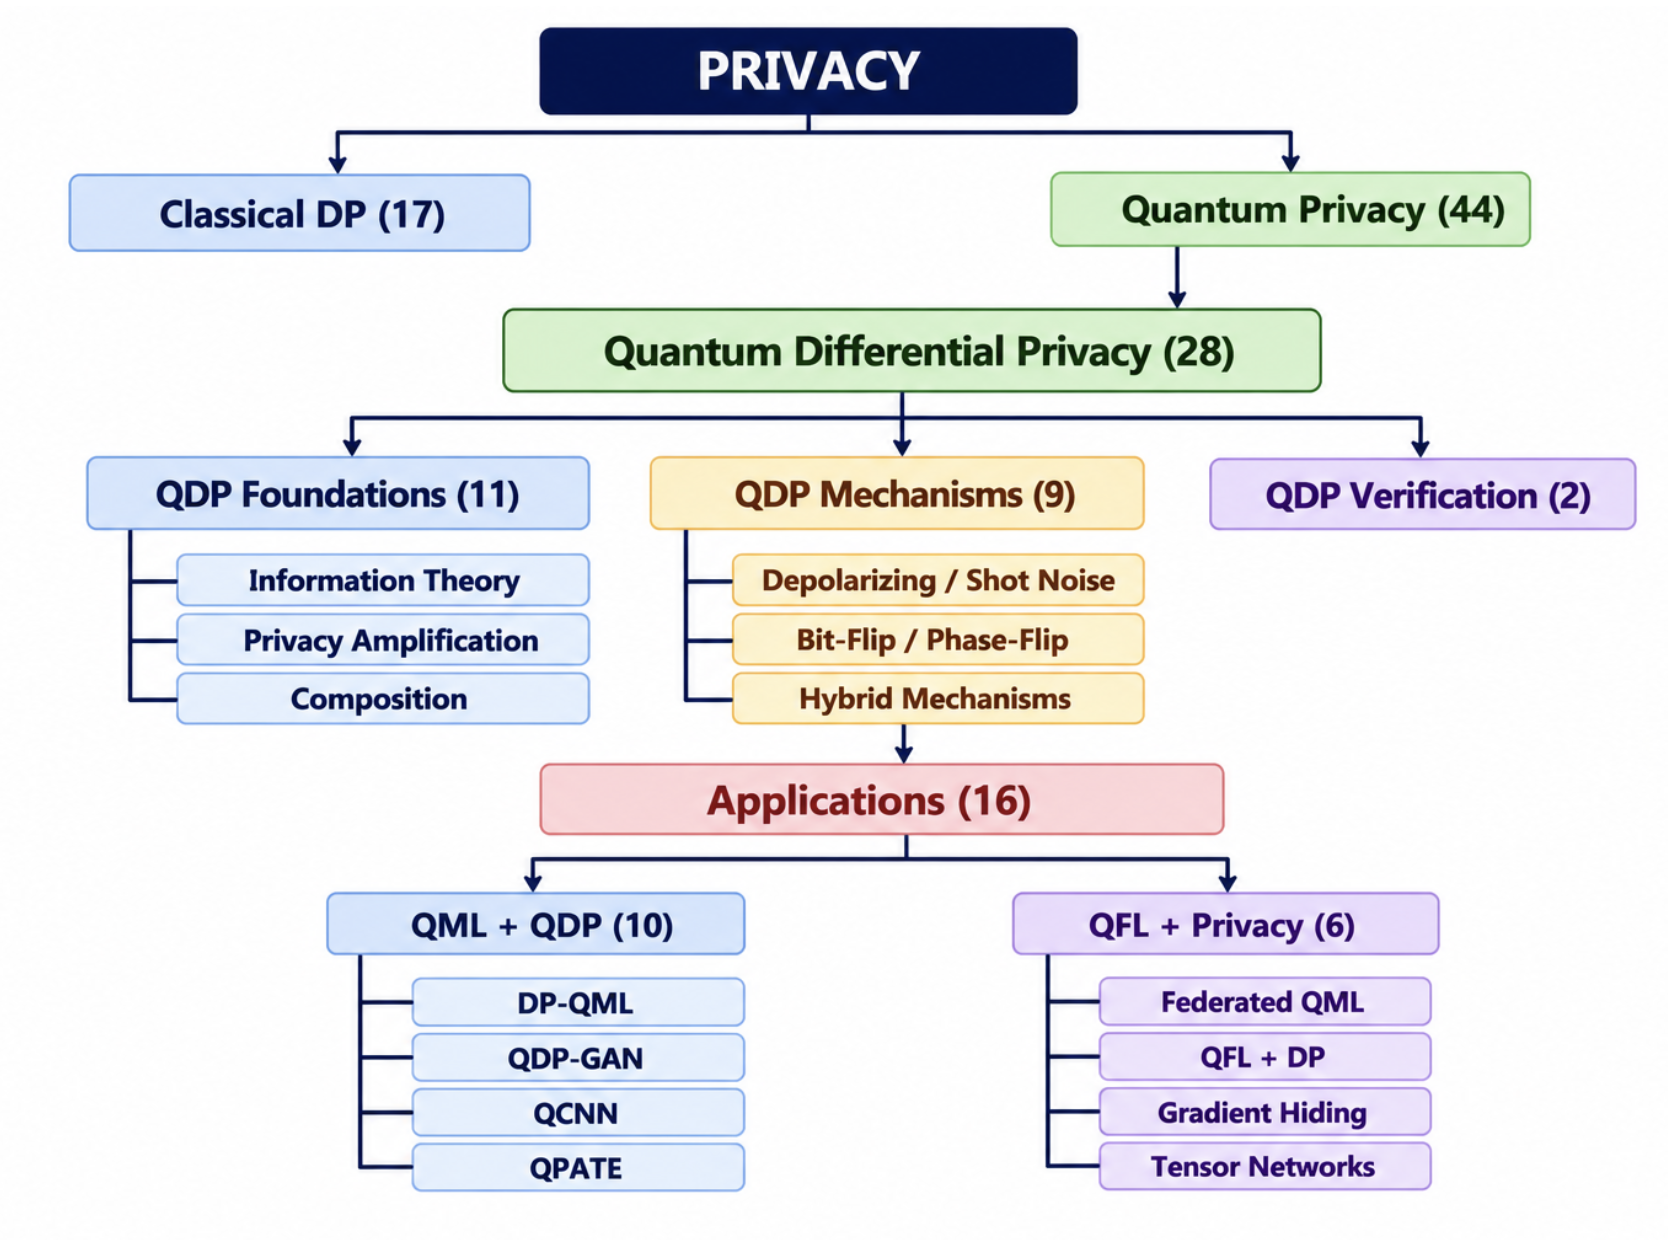
\includegraphics[width=\textwidth]{state_of_qdp.png}
    \caption{State of the art of quantum differential privacy (own elaboration, based on the literature review described above).}
    \label{fig:state_of_qdp}
\end{figure*}

As shown in Figure~\ref{fig:state_of_qdp}, the investigation yielded positive results as there were many academic papers that not only mentioned the topic but gave valuable research and insight on possible angles the project could leap into. Among the most interesting ones are: \cite{watkins2023quantum} in which a hybrid quantum machine learning framework was proposed to allow differential privacy in the model. \cite{song2025hybrid} which tested different quantum differential privacy mechanisms along with proposing its own \textbf{Lifted} quantum differential privacy, which enhanced the randomness induced in the quantum states. \cite{yang2023improved} in which an extended analysis was made to characterize the protection quantum noise can offer in the setting of quantum-classical algorithms. Finally, in the study of Zhou and Ying~\cite{zhou2017differential}, they define a framework of differential privacy in the quantum setting and examine how different noise mechanisms change the protection of a privacy budget $\epsilon$.

\section{Data Processing and Analysis}
\label{sec:data_processing_and_analysis}

This section details the data processing and analysis methodology that was used in order to prepare the classical Statlog (German Credit Data) dataset~\cite{hofmann1994german, germancredit2026} for use in the quantum setting. Firstly, we outline the dataset characteristics, then the variable selection procedures and, lastly, the quantum encoding procedures for the selected data. 

\subsection{Dataset description}

The selected dataset for this investigation is the Statlog (German Credit Data) dataset created by Professor Hans Hofmann \cite{hofmann1994german}. This multivariate dataset aims to classify people as a good or bad credit risk. The original dataset is composed of 1000 instances that span 21 variables (7 numerical, 13 categorical, and the target). 

In the original dataset created by Professor Hofmann, all non-numerical variables use an attribute code to define their characteristics (e.g., the status of a person whose checking account is less than 0 Deutsche Marks (DM) is A11). For that reason, it was decided that the investigation was going to use a curated version of the dataset \cite{germancredit2026} which transforms all the labels to their definition as a means of simplifying the readers' understanding of the dataset by eliminating that intermediate layer of label and category. Every mention of the dataset henceforth will refer to this curated version and not the original compiled by Professor Hofmann.

A simple data analysis concluded that the dataset did not have any problem in terms of completeness (as all rows include all 21 variables) or uniqueness (as there is no instance of an exact duplicate). For these reasons, no special cleaning procedure was done prior to variable selection.

\subsection{Variable selection with PhiK}
\label{subsec:var_selection}

In order to hold quantum data for a dataset that contains 1000 instances of 20 variables each, the simulation would, at a maximum, store 1000 $2^n \times 2^n$ density matrices, with $n$ being the number of qubits used. This means that using the full 20 variables, one per qubit, would imply $2^{20} \times 2^{20} \approx 1.1 \times 10^{12}$ complex entries, and at 16 bytes each, that is about 16 TiB per matrix. It was decided that a correlation study over the target variable would be an adequate way to reduce this load. The reasons for this decision are: First, the investigation did not aim to produce a classifier and thus could use a smaller number of variables in the experiments. Second, the variables selected from a correlation study would be the most likely candidates to be chosen as significant by a classifier.

As mentioned previously, however, most of the variables in this dataset are not numeric and thus a popular correlation analysis such as the Pearson correlation is not an adequate choice to evaluate variable correlation. For starters, for a nominal variable the Pearson coefficient relies on an arbitrary choice for the label and since the proportions of the target variable in the dataset for each category are not the same across the board, a change in category label implies a change in the coefficient. Moreover, the Pearson coefficient identifies linear relationships between variables well but fails for nonlinear cases.

For these reasons it was decided to use the PhiK method \cite{BAAK2020107043PHIK} to select the variables which show a consistently stronger correlation with the target variable. PhiK is a stronger candidate as it works well for both numerical and categorical variables and it is able to identify nonlinear relationships between them.

We used Baak et al.'s PhiK library to measure the correlation and significance between each variable and the target and recorded the results in Table~\ref{tab:phik}. It is important to note that the library returns, for a pair of variables, two results: the first is $\phi_{K}$ which is the measurement of how strong the relationship between the two variables is. This result is calculated by calibrating a $\chi^2$ test statistic to a contingency table (populated with the categorical variables or binned numerical variables) with respect to a bivariate normal distribution. This calibration returns a $\phi_{K}$ with range of 0 (no association) to 1 (complete association). Since $\phi_{K}$ depends on the counts of the contingency table, renumbering the categories no longer affects the end result. The second result is $Z$ which is a conversion of the p-value from the independence test into a number of standard deviations. A higher $Z$ provides more evidence that the variable is not independent from the target.

\begin{table}[htbp]
  \caption{$\phi_K$ correlation of each feature with the target and its statistical significance with a cutoff of $Z > 2.81$.}
  \label{tab:phik}
  \centering
  \begin{tabular}{lrrc}
    \toprule
    Feature & $\phi_K$ & $Z$ & Significant \\
    \midrule
    \texttt{status\_account}           & 0.512 & 10.965       & Yes \\
    \texttt{credit\_history}           & 0.197 & 6.912        & Yes \\
    \texttt{month\_duration}           & 0.285 & 5.648        & Yes \\
    \texttt{status\_savings}           & 0.147 & 5.283        & Yes \\
    \texttt{credit\_amount}            & 0.241 & 4.388        & Yes \\
    \texttt{collateral}                & 0.217 & 4.009        & Yes \\
    \texttt{purpose}                   & 0.204 & 3.715        & Yes \\
    \texttt{housing}                   & 0.077 & 3.601        & Yes \\
    \texttt{years\_employment}         & 0.098 & 3.053        & Yes \\
    \texttt{other\_installment\_plans} & 0.063 & 2.891        & Yes \\
    \texttt{is\_foreign\_worker}       & 0.109 & 2.545        & No  \\
    \texttt{age}                       & 0.142 & 2.177        & No  \\
    \texttt{status\_and\_sex}          & 0.123 & 1.953        & No  \\
    \texttt{secondary\_obligor}        & 0.041 & 1.835        & No  \\
    \texttt{payment\_to\_income\_ratio}& 0.075 & 1.045        & No  \\
    \texttt{telephone}                 & 0.021 & 0.689        & No  \\
    \texttt{n\_credits}                & 0.000 & 0.043        & No  \\
    \texttt{job}                       & 0.000 & $-0.390$     & No  \\
    \texttt{residence\_since}          & 0.000 & $-1.070$     & No  \\
    \texttt{n\_guarantors}             & 0.000 & $-\infty$    & No  \\
    \bottomrule
  \end{tabular}
\end{table}

For the variable selection we chose to use $Z$ because, although $\phi_{K}$ measures the correlation between variables, the significance $Z$ of that correlation indicates whether that correlation is significant enough to be told apart from chance. The Bonferroni method states that, to ensure that the probability of at least one false positive across $k$ tests (in our case $k = 20$ for $20$ variables against the target) is at most $\alpha = 0.05$, each individual test must use a significance level of $\alpha' = \alpha/k = 0.05/20 = 0.0025$ \cite{bland1995multiple}. Here a false positive is a variable that is independent of the target but is selected anyway. Since $\alpha' = 0.0025$ corresponds to $Z \approx 2.81$, we used $Z > 2.81$ as the cutoff for the selection of the variables.

%Table~\ref{tab:phik} has the values that the PhiK method returned for all 20 variables with regards to the target sorted by $Z$. As an example the reader can observe that the variable \textbf{housing} has a small correlation with target yet a strong significance. On the contrary \textbf{age} has a higher correlation than \textbf{housing} with target yet a small enough significance to not merit its selection

As the reader can observe in Table~\ref{tab:phik}, the selection took 10 out of the 20 variables, which, as mentioned before, now leaves a maximum of 1000 $2^{10} \times 2^{10}$ matrices as opposed to 1000 $2^{20} \times 2^{20}$ should we use one qubit per variable. We will show how we lowered that number in Section~\ref{subsec:encoding_variables}. The definition and type of each variable is recorded in Appendix~\ref{ap:selected_features}.

\subsection{Encoding of classical variables into quantum}
\label{subsec:encoding_variables}

Having chosen a reduced set of variables from the dataset (10 from the original 20), the next step was to encode the classical information from each variable into qubits which could be used in the quantum simulation. For this it is important to note that the variables were divided into two groups, each with its own encoding:

\subsubsection{Categorical Variables}

These are categorical variables whose categories do not follow a natural ranking. An example of this is the variable \texttt{purpose}, which has ten categories (car (new), vacation, education, among others). As the reader can observe, these categories do not follow a natural order, as there is no way to tell if, say, car goes before or after education. Due to this, it was decided to separate them from the categorical (ordinal) variables that will be mentioned later on.

The proposed encoding for these types of variables is given by Definition~\ref{def:encoding_categorical}.

\begin{definition}
  (Method for encoding categorical variables). For a categorical variable with $K$ categories, when encoding the label $c \in \{0, \dots, K - 1\}$, the resulting encoded qubit state $\ket{\psi}$ is given by the equation

  \[
    \ket{\psi} = RZ(\phi)H\ket{0} \quad \text{with} \quad \phi = \frac{2\pi c}{K}
  \]
  \label{def:encoding_categorical}
\end{definition}


This encoding ends up with a qubit state in one of $K$ equally distributed points across the equator of the Bloch sphere. We choose to place the qubit on the equator because, from Definition~\ref{def:trace_distance_vector}, we can express $\tau$ in terms of the angle between two points of a circle $\Delta$ and the radius of that circle as $r\sin{\frac{\Delta}{2}}$. With this expression the reader can note that the minimum distance $\tau$ is maximized for all other angles on the sphere when the radius is maximum, which happens at the equator of the sphere. Moreover, one could argue that having a smaller $\theta$ (i.e., the angle of rotation about the y-axis of the Bloch sphere) would reduce $\epsilon$, and one would be right if not for the fact that it comes with the tradeoff of making the categories less distinguishable. In the case where $\theta = 0$, any rotation over the z-axis would be invalidated, since without a rotation over the y-axis it would only add a global phase.

This method assures then that $\tau$ between two categories is at least $\sin(\frac{\pi}{K})$. What this means in theory is that the privacy in the local setting will not change the final $\epsilon$, as regardless of the labels given to any category, the angle between the labels themselves might change, but the possible angles between different categories will remain the same. However, what this encoding does not prevent is the fact that different categories can have different proportions. The labels given to each category can impact the distance $\tau$ between the dataset and that same dataset without a person included, which, as will be explained in Section~\ref{sec:finding_epsilon}, is crucial when computing $\epsilon_{exp}$ and $\epsilon_{theo}$ and therefore, in theory, can lead to different results. In Appendix~\ref{ap:label_categorical} we compiled the $c$ values given to each variable's categories.

\subsubsection{Numerical and ordinal variables}

These are variables which are either ranges of an amount (ordinal) or numerical. An example of these variables is \texttt{month\_duration}, which gives the loan's duration in months. A loan that goes for 4 months is clearly shorter than a loan that goes for 72, thus it is important to preserve that order. The encoding method which we believed would be able to preserve this order was dense angle encoding~\cite{ibm_encoding}.

The question that remained, however, was: which variables were going to be encoded together? To answer this question we first created all 15 possible arrangements of the 5 numerical and ordinal variables into two pairs and a single variable. Then, we once again used the PhiK method to analyze the correlation between each pair of variables which is documented in Table~\ref{tab:phik_numerical_ordinal} (Appendix~\ref{ap:phik_numerical_ordinal}). From this small investigation it was concluded that the combination of variables that yielded the smallest correlation in the worst case was \texttt{status\_account} as the lone variable, \texttt{status\_savings} and \texttt{month\_duration} as the first pair, and \texttt{years\_employment} and \texttt{credit\_amount} as the second pair. We chose this combination as the smallest correlation between the worst pair would imply that the qubits carried as little redundant information within each qubit as possible.

Before the encoding definition, we defined a function \textbf{minmax}(min, max, a), which normalizes a value $a \in [min , max]$ to $a \in [0 , \pi ]$. 

\begin{definition}
  (Min-max normalization). Given a value $a \in [min , max]$ with $min, max \in \mathbb{R}$ we define the function \textbf{minmax} as

  \[
    \textbf{minmax(min, max, a)} = \pi \times \frac{a-min}{max-min}
  \]
  \label{def:minmax}
\end{definition}

With this definition the method to encode numerical and ordinal variables is dense angle encoding~\cite{ibm_encoding}, which we define as:

\begin{definition}
  (Method for encoding numerical and ordinal variables with dense angle encoding). For an ordinal variable with $K$ categories and a numerical variable with range $[n_{Min}, n_{Max}]$, when encoding the ordinal variable with label $c \in \{0, \dots, K-1\}$ and the numerical variable with value $n \in [n_{Min}, n_{Max}]$, the resulting dense angle encoding is given by
  
  \begin{align*}
    \ket{\psi} &= RZ(\phi)RY(\theta)\ket{0},\\
    \text{with } \phi &= minmax(n_{Min}, n_{Max}, n),\\
    \text{and } \theta &= minmax(-0.5, K - 0.5, c)
  \end{align*}
  \label{def:encoding_dense_angle}
\end{definition}

Because of the pairing selection, the definition only needs to cover the case where an ordinal variable is paired with a numerical one. Thus it is important to note that the reason \textbf{minmax} is calibrated from $-0.5$ to $K-0.5$ for the ordinal variables is so that the resulting categories cannot reach the poles, which would result in the gate RZ being invalidated. This calibration then sets each category into the middle of a bin of length $\frac{\pi}{K}$. An exception to this definition is the lone variable \texttt{status\_account}, since it does not need this calibration as there is no RZ gate to invalidate, so the range for \textbf{minmax} is $[0, K-1]$. 

As the reader can observe, thanks to dense angle encoding we can actually reduce the number of qubits necessary for encoding the full 10 variables to 8 which helps reduce the computational toll from the original $2^{10}\times 2^{10}$ matrices with a 1:1 qubit-to-variable encoding to $2^{8}\times 2^{8}$ matrices. The final quantum circuit can be seen in Figure~\ref{fig:quantum_encoding_circuit}.

\begin{figure}[!t]
  \centering
  \footnotesize
  \begin{quantikz}[row sep=0.25cm, column sep=0.3cm]
    \lstick{\texttt{collateral}~~$\ket{0}$}              & \gate{H}          & \gate{R_Z(2\pi c/K)} & \qw \\
    \lstick{\texttt{purpose}~~$\ket{0}$}                 & \gate{H}          & \gate{R_Z(2\pi c/K)} & \qw \\
    \lstick{\texttt{credit\_history}~~$\ket{0}$}         & \gate{H}          & \gate{R_Z(2\pi c/K)} & \qw \\
    \lstick{\texttt{housing}~~$\ket{0}$}                 & \gate{H}          & \gate{R_Z(2\pi c/K)} & \qw \\
    \lstick{\texttt{other\_installment\_plans}~~$\ket{0}$} & \gate{H}        & \gate{R_Z(2\pi c/K)} & \qw \\
    \lstick{\shortstack[r]{\texttt{status\_savings}\\\texttt{month\_duration}}~~$\ket{0}$}     & \gate{R_Y(\theta)} & \gate{R_Z(\phi)} & \qw \\
    \lstick{\shortstack[r]{\texttt{years\_employment}\\\texttt{credit\_amount}}~~$\ket{0}$}    & \gate{R_Y(\theta)} & \gate{R_Z(\phi)} & \qw \\
    \lstick{\texttt{status\_account}~~$\ket{0}$}         & \gate{R_Y(\theta)} & \qw                 & \qw
  \end{quantikz}
  \caption{8-qubit encoding circuit for the 10 selected variables}
  \label{fig:quantum_encoding_circuit}
\end{figure}

\section{Finding the experimental privacy budget}
\label{sec:finding_epsilon}

Before starting with the in-depth explanation of each experiment it is important to mention the noise parameters chosen for all the different mechanisms mentioned in Section~\ref{sec:background}; these are compiled in Table~\ref{tab:noise_params}. All of these parameters are just that, parameters, so the selection was made mainly as a way to, firstly, execute all the tests with the same parameters and thus allow for a comparison between experiments and, secondly, abide by the restrictions imposed on $\lambda$ and $\gamma$ by Theorem~\ref{thm:epsilon_pad} and on $\eta$ by Theorem~\ref{thm:epsilon_gad}. Furthermore, due to the nature of the PAD mechanism, it was important to choose a $\lambda \in (0, 0.5)$ to allow the mechanism to behave differently from GAD and DEP.

\begin{table}[H]
  \caption{Selection of parameters for noise mechanisms}
  \label{tab:noise_params}
  \centering
  \begin{tabular}{ll}
    \toprule
    Mechanism & Parameters\\
    \midrule
    Depolarizing & $p = 0.5$ \\
    Generalized Amplitude Damping & $\eta = 0.5$, $\gamma = 0.5$ \\
    Phase-Amplitude Damping & $\eta = 0.5$, $\gamma = 0.5$, $\lambda = 0.25$ \\
    \bottomrule
  \end{tabular}
\end{table}

\subsection{Central Setting}
\label{subsec:experiment_central_setting}

The first experiment that was carried out was finding the $\epsilon_{theo}$ and $\epsilon_{exp}$ in a central setting for each qubit $k$ of the dataset (recall the encoding from Section~\ref{subsec:encoding_variables}). In other words, we wanted to see what privacy guarantee each of the mechanisms $\mathcal{M}_{GAD}$, $\mathcal{M}_{PAD}$ and $\mathcal{M}_{DEP}$ provided. In order to accomplish this, we designed the pipeline documented in Figure~\ref{fig:central_setting}.

\begin{figure*}[!t]
  \centering
  \resizebox{\textwidth}{!}{%
  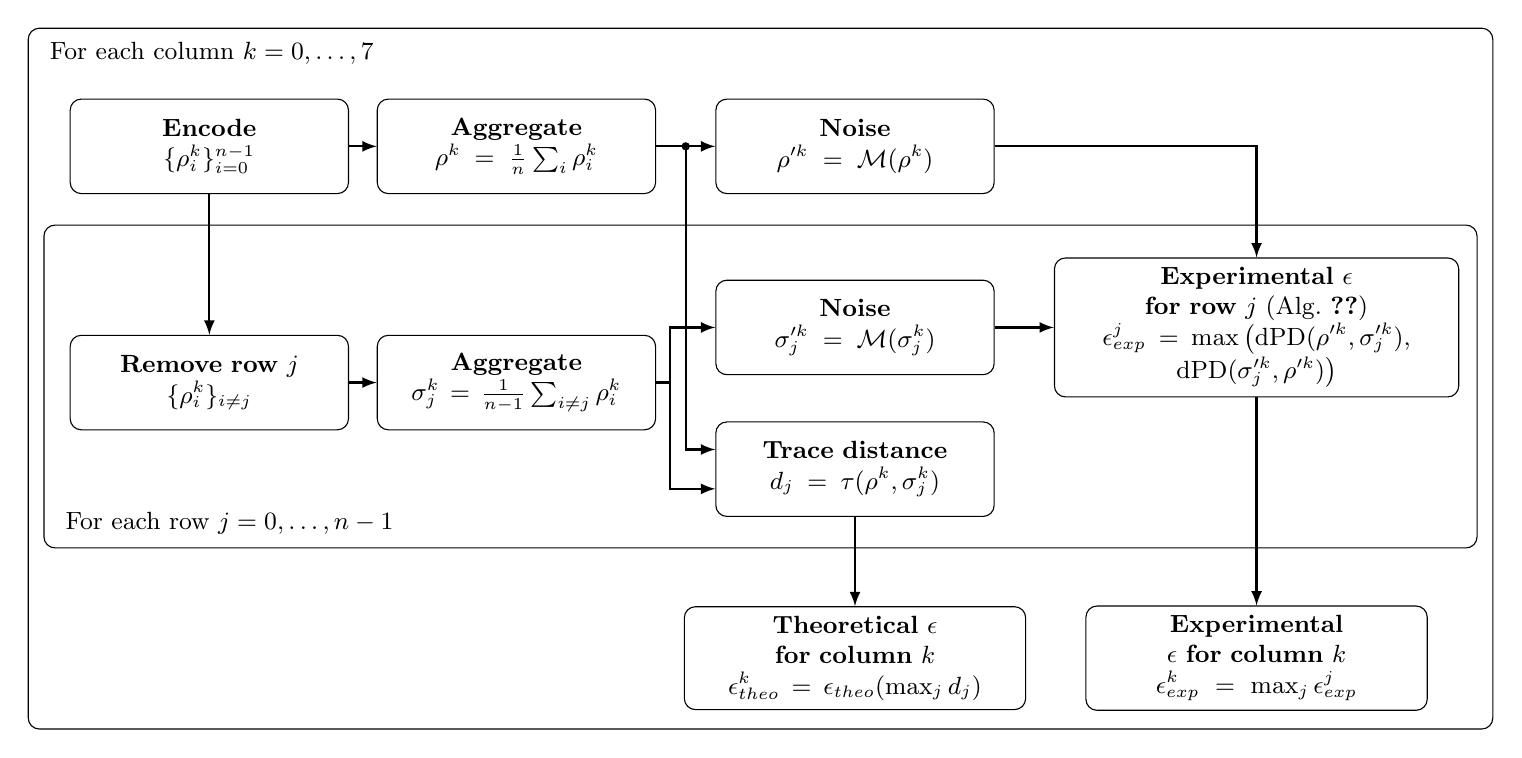
\begin{tikzpicture}[
      font=\small,
      box/.style={draw, rounded corners, align=center, text width=3.3cm, minimum height=1.2cm},
      arr/.style={-latex, thick}
    ]
    % loop frames
    \draw[rounded corners] (0.3,1.5) rectangle (18.9,-7.4);
    \node[anchor=north west] at (0.45,1.45) {For each column $k = 0, \dots, 7$};
    \draw[rounded corners] (0.5,-1.0) rectangle (18.7,-5.1);
    \node[anchor=south west] at (0.65,-5.05) {For each row $j = 0, \dots, n-1$};
    % full dataset
    \node[box] (enc) at (2.6,0) {\textbf{Encode}\\ $\{\rho_i^k\}_{i=0}^{n-1}$};
    \node[box] (agg) at (6.5,0) {\textbf{Aggregate}\\ $\rho^k = \frac{1}{n}\sum_{i}\rho_i^k$};
    \node[box] (noise) at (10.8,0) {\textbf{Noise}\\ $\rho^{\prime k} = \mathcal{M}(\rho^k)$};
    % neighboring dataset
    \node[box] (rem) at (2.6,-3.0) {\textbf{Remove row $j$}\\ $\{\rho_i^k\}_{i \neq j}$};
    \node[box] (aggs) at (6.5,-3.0) {\textbf{Aggregate}\\ $\sigma_j^k = \frac{1}{n-1}\sum_{i \neq j}\rho_i^k$};
    \node[box] (noises) at (10.8,-2.3) {\textbf{Noise}\\ $\sigma_j^{\prime k} = \mathcal{M}(\sigma_j^k)$};
    \node[box] (dist) at (10.8,-4.1) {\textbf{Trace distance}\\ $d_j = \tau(\rho^k, \sigma_j^k)$};
    \node[box, text width=4.9cm] (epsj) at (15.9,-2.3) {\textbf{Experimental $\epsilon$ for row $j$} (Alg.~\ref{alg:dpd})\\ $\epsilon_{exp}^{j} = \max\big(\mathrm{dPD}(\rho^{\prime k}, \sigma_j^{\prime k}),$\\ $\mathrm{dPD}(\sigma_j^{\prime k}, \rho^{\prime k})\big)$};
    % per-column results
    \node[box, text width=4.1cm] (theo) at (10.8,-6.5) {\textbf{Theoretical $\epsilon$ for column $k$}\\ $\epsilon_{theo}^{k} = \epsilon_{theo}(\max_j d_j)$};
    \node[box, text width=4.1cm] (expk) at (15.9,-6.5) {\textbf{Experimental $\epsilon$ for column $k$}\\ $\epsilon_{exp}^{k} = \max_j \epsilon_{exp}^{j}$};
    % arrows
    \draw[arr] (enc) -- (agg);
    \draw[arr] (agg) -- (noise);
    \draw[arr] (enc) -- (rem);
    \draw[arr] (rem) -- (aggs);
    \draw[arr] (noise.east) -| (epsj.north);
    \draw[arr] (noises) -- (epsj);
    \draw[arr] (aggs.east) -- (8.45,-3.0) |- (noises.west);
    \draw[arr] (8.45,-3.0) |- ([yshift=-0.25cm]dist.west);
    \fill (8.65,0) circle (1.5pt);
    \draw[arr] (8.65,0) |- ([yshift=0.25cm]dist.west);
    \draw[arr] (dist) -- (theo);
    \draw[arr] (epsj) -- (expk);
  \end{tikzpicture}%
  }
  \caption{Experimental pipeline for finding $\epsilon_{exp}$ and $\epsilon_{theo}$}
  \label{fig:central_setting}
\end{figure*}

The pipeline begins by calculating some values that will be used during the leave-one-out loop: encoding the full column using the methodology provided in Section~\ref{sec:data_processing_and_analysis}, which will become our set $\{\rho_i^{k}\}$, containing the states of each person in the dataset for that column. That complete set will be aggregated into a single matrix $\rho^{k}$, which will hold an average of all the participants of the dataset for the column $k$. Then noise from the selected noise mechanism will be applied to that density matrix, resulting in the matrix $\rho'^{k}$. With those two matrices calculated, the pipeline will begin a loop that iterates over each participant of the dataset in order to compare the original against a leave-one-out version of the dataset where the row $j$ is removed.

For each row $j$, the process is as follows: aggregate the set $\{\rho_i^{k}\}$ with the row $j$ removed, which results in the density matrix $\sigma_j^{k}$, the aggregation of all participants except $j$. From $\sigma_j^{k}$ both $\sigma_j^{\prime k}$ and $d_j$ will be calculated. $\sigma_j^{\prime k}$ is the density matrix that results from applying the selected noise mechanism to $\sigma_j^{k}$, and $d_j$ is the trace distance between $\rho^{k}$ and $\sigma_{j}^{k}$, which has to be calculated with the pre-noise matrices as per Theorems~\ref{thm:epsilon_gad} through~\ref{thm:epsilon_dep}. Lastly, it will calculate $\epsilon_{exp}^{j}$, which is the $\epsilon_{exp}$ for the $j$-th row and corresponds to the maximum of the values that Algorithm~\ref{alg:dpd} returns in both directions. 

With all those values, the only remaining step of the pipeline is to input them into each method for finding $\epsilon$. On the theoretical side, the pipeline will input the maximum trace distance and the noise mechanism's parameters into one of the theorems defined in Section~\ref{sec:background} (for the depolarizing mechanism $D=2$, as we are calculating on a per-qubit basis) for the resulting $\epsilon_{theo}$ of the column. In the case of $\epsilon_{exp}$, it is the maximum $\epsilon_{exp}^{j}$ over all rows $j$, as that is the maximum privacy loss that the dataset can offer for that noise mechanism.

With the $\epsilon_{exp}^{k}$ and $\epsilon_{theo}^{k}$ calculated for each column $k$ of the dataset, the only thing that remains is to add them to find the upper bound of $\epsilon_{exp}$ and $\epsilon_{theo}$ of the dataset. In the pipeline, the curator would release the noisy density matrices for the 8 qubits
\[
  \bigotimes_{k=0}^{7} \rho^{\prime k} = \bigotimes_{k=0}^{7} \mathcal{M}(\rho^{k}).
\]
Because of Lemma~\ref{lem:product_channel}, this is equal to
\[
  \Big(\bigotimes_{k=0}^{7} \mathcal{M}\Big)\Big(\bigotimes_{k=0}^{7} \rho^{k}\Big) = \mathcal{M}_{[8]}(\rho^{0}, \dots, \rho^{7})
\]
which is the combination defined in Corollary~\ref{cor:composition}, and thus the addition is valid.
 

\begin{lemma}
  For $i = 1, \dots, k$, let $\mathcal{E}_i(\rho) = \sum_{a} E_{i,a}\, \rho\, E_{i,a}^{\dagger}$ be a quantum operation on $\mathcal{H}_i$ and $\rho_i$ a density operator on $\mathcal{H}_i$. Then
  \[
    \Big(\bigotimes_{i=1}^{k} \mathcal{E}_i\Big)\Big(\bigotimes_{i=1}^{k} \rho_i\Big) = \bigotimes_{i=1}^{k} \mathcal{E}_i(\rho_i).
  \]
  \label{lem:product_channel}
\end{lemma}

For readability, the proof of Lemma~\ref{lem:product_channel} is deferred to Appendix~\ref{ap:composition_proof}.

In the case of the depolarizing mechanism, we can actually modify the pipeline by removing the need to encode each column individually and applying the noise to the full 8 columns, since Theorem~\ref{thm:epsilon_dep} allows it. This, however, is classified as a separate experiment, since both the aggregation and the release that the curator would perform are over the full 8-qubit matrix (not per qubit, as was explained), thus not allowing for a comparison against the original pipeline. Later on, in Section~\ref{sec:discussion_and_conclusion}, we will discuss how these methods yield very different privacy results.


\subsection{Local Setting}
\label{subsec:experiment_local_setting}

We have now considered an experiment where a trusted curator applies the noise to the data and releases the data. This experiment, however, tries to answer the question of what would happen if it were each individual person applying the noise, the local setting.

In the central setting we defined neighbors as two aggregated density matrices, the one for the full 1000 $\rho$ rows and the leave-one-out $\sigma$. In this setting (inspired by~\cite[Def.~12.1]{dwork2014algorithmic} as mentioned in Section~\ref{sec:background}), however, since it is just one person at a time who is privatizing their data, it would not make sense to compare two different people as neighbors, as in reality what the attacker would want to know is ``what was person A's original category?''. With this idea, this experiment defines the neighbors as the possible states that each label is encoded into, and because of Definition~\ref{def:qdp} we can compare two states as neighbors by their trace distance $\tau$. This experiment, however, limits the variables we can encode. As mentioned in Section~\ref{subsec:encoding_variables} the numerical variables need to be normalized within the Bloch sphere with the minimum and maximum values of the variables. In the local setting a single person has no way to access that data and thus cannot encode it in that manner. With that limitation in mind, this setting calculates the $\epsilon$ for all the categorical variables and the sole variable \texttt{status\_account} since the other two ordinal variables are accompanied in the same qubit by a numerical variable and thus cannot be encoded independently. Figure~\ref{fig:local_setting} shows the pipeline for the local setting experiment.
\begin{figure*}[!t]
  \centering
  \resizebox{\textwidth}{!}{%
  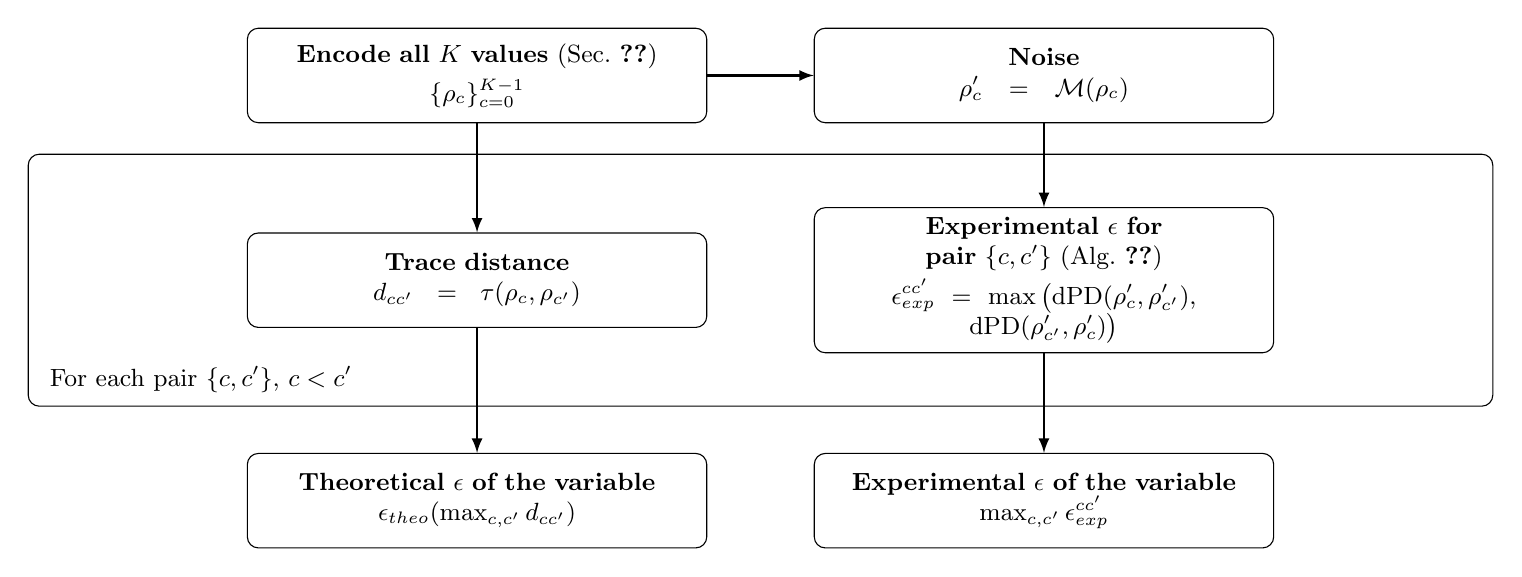
\begin{tikzpicture}[
      font=\small,
      box/.style={draw, rounded corners, align=center, text width=5.6cm, minimum height=1.2cm},
      arr/.style={-latex, thick}
    ]
    % pair-loop frame (same width as Fig.~\ref{fig:central_setting}, so both figures share one scale)
    \draw[rounded corners] (0.3,-1.0) rectangle (18.9,-4.2);
    \node[anchor=south west] at (0.45,-4.15) {For each pair $\{c, c'\}$, $c < c'$};
    % all values of the variable
    \node[box] (enc) at (6.0,0) {\textbf{Encode all $K$ values} (Sec.~\ref{subsec:encoding_variables})\\[3pt] $\{\rho_c\}_{c=0}^{K-1}$};
    \node[box] (noise) at (13.2,0) {\textbf{Noise}\\ $\rho^{\prime}_c = \mathcal{M}(\rho_c)$};
    % pair of values
    \node[box] (dist) at (6.0,-2.6) {\textbf{Trace distance}\\ $d_{cc'} = \tau(\rho_c, \rho_{c'})$};
    \node[box] (epsp) at (13.2,-2.6) {\textbf{Experimental $\epsilon$ for pair $\{c, c'\}$} (Alg.~\ref{alg:dpd})\\[2pt] $\epsilon_{exp}^{cc'} = \max\big(\mathrm{dPD}(\rho^{\prime}_c, \rho^{\prime}_{c'}),$\\ $\mathrm{dPD}(\rho^{\prime}_{c'}, \rho^{\prime}_c)\big)$};
    % results for the variable
    \node[box] (theo) at (6.0,-5.4) {\textbf{Theoretical $\epsilon$ of the variable}\\ $\epsilon_{theo}(\max_{c,c'} d_{cc'})$};
    \node[box] (expk) at (13.2,-5.4) {\textbf{Experimental $\epsilon$ of the variable}\\ $\max_{c,c'} \epsilon_{exp}^{cc'}$};
    % arrows
    \draw[arr] (enc) -- (noise);
    \draw[arr] (enc) -- (dist);
    \draw[arr] (noise) -- (epsp);
    \draw[arr] (dist) -- (theo);
    \draw[arr] (epsp) -- (expk);
  \end{tikzpicture}%
  }
  \caption{Pipeline for the local setting experiment for finding $\epsilon$ for a categorical or ordinal variable} 
  \label{fig:local_setting}
\end{figure*}

The experiment begins by defining two sets $\{\rho_c\}$ which are all the density matrices that result from encoding the $c$-th label and $\{\rho_c^{\prime}\}$ which is the set of all the density matrices $\rho_c$ that have been passed over the noise mechanism $\mathcal{M}$. Then, for each pair of labels $\{c, c^{\prime}\}, c < c^{\prime}$, we calculate both the trace distance between the original noiseless density matrices $\rho_c$ and $\rho_{c^{\prime}}$ and the $\epsilon_{exp}$ which is the same procedure as the central setting just with inputs $\rho_c^{\prime}$ and $\rho_{c^{\prime}}^{\prime}$. Then, at the end, we make the same search for the maximum $\epsilon_{theo}$ and $\epsilon_{exp}$ of all the analyzed pairs and that is the final result of the variable. 


\section{Measurement and Classical release of a categorical variable}
\label{sec:measurement_release}

With the previous two experiments we have been able to find $\epsilon_{theo}$ and $\epsilon_{exp}$ for both settings of differential privacy. This, however, leaves one important question to answer: what does this privacy budget actually look like after the classical release of the data? The previous experiments did not need to answer this question to compute $\epsilon$, as we had the full distribution (density matrix) of the qubits.

To answer this question, we first need to clarify the concept of a \textbf{copy}. For the purposes of this investigation, a copy is one qubit in a specific quantum state, either a pure state $\ket{\psi}$ or a mixed state with density matrix $\rho$. When that copy is measured, it collapses into one of the two states of the measurement basis (i.e., $\ket{+}$ or $\ket{-}$ for the $X$ basis). Because of the no-cloning theorem~\cite{watrous_limitations}, the curator (or anybody, for that matter) cannot save the state prior to the measurement to measure it again, and thus every new measurement requires the state to be fully prepared again.

Figure~\ref{fig:release_designs} shows what happens to the data after the pipelines of Subsections~\ref{subsec:experiment_central_setting} and~\ref{subsec:experiment_local_setting}. In the central setting, the final state is the aggregation of the full dataset, $\rho = \frac{1}{n}\sum_{i=1}^{n}\rho_i$, so by the law of total probability, measuring a copy of $\rho^{\prime}$ is no different from drawing a random person $i$ and then measuring their state. In other words, every person is hidden within the full aggregation, and the privacy of each copy is the $\epsilon$ calculated in Subsection~\ref{subsec:experiment_central_setting}. However, each new copy needed to estimate the distribution is another draw and thus costs another $\epsilon$, resulting in a total of $N\epsilon$ because of Corollary~\ref{cor:composition}, with $N$ being the number of copies measured. In the local setting, on the other hand, each individual only needs a single measurement. Since a measurement (Definition~\ref{def:quantum_measurement}) can be thought of as a quantum operation in itself, Proposition~\ref{prop:post_processing} implies that the final $\epsilon$ is at most the one found in the local setting experiment. 

\begin{figure*}[!t]
  \centering
  \resizebox{\textwidth}{!}{%
  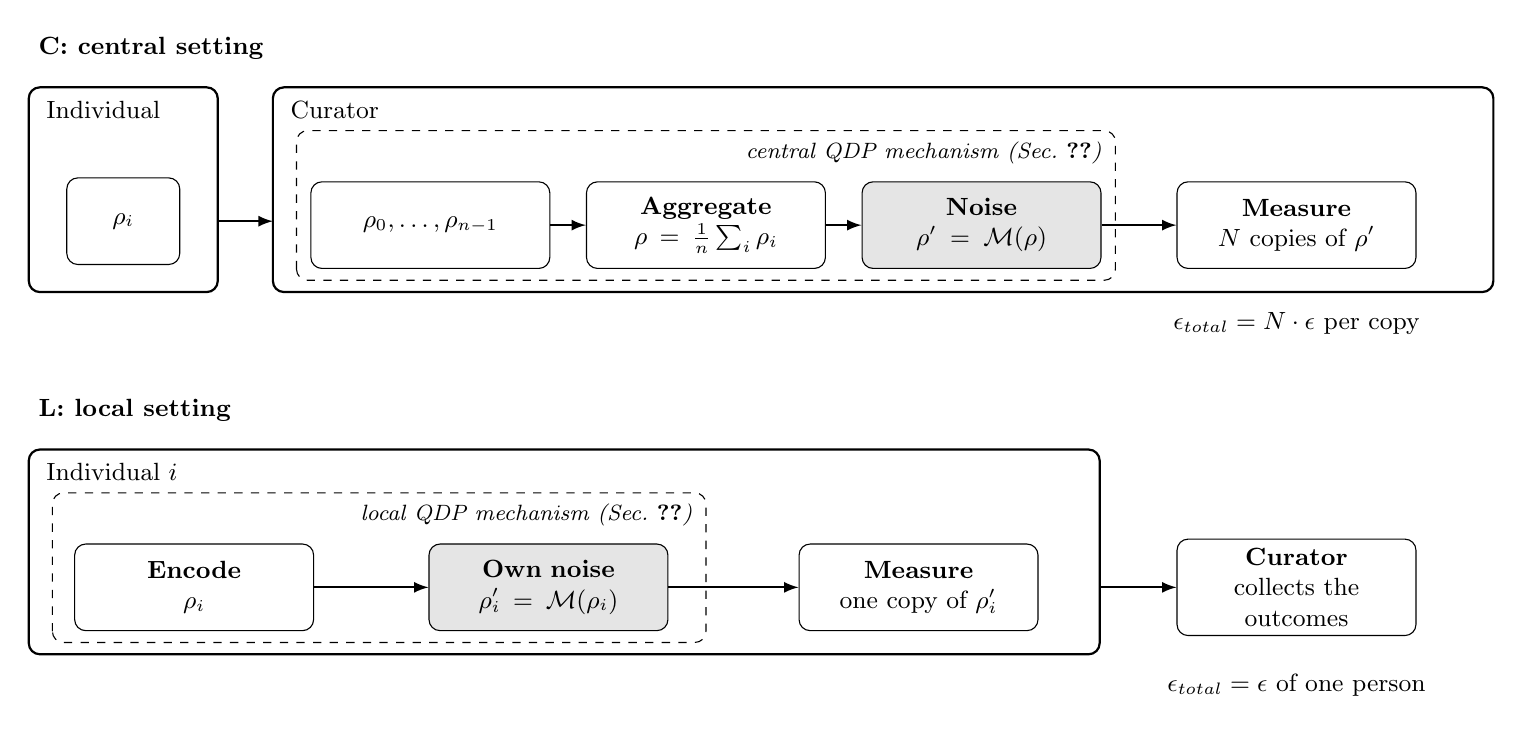
\begin{tikzpicture}[
      font=\small,
      box/.style={draw, rounded corners, align=center, text width=2.8cm, minimum height=1.1cm, fill=white},
      noisebox/.style={box, fill=gray!20},
      group/.style={draw, rounded corners, thick},
      mech/.style={draw, rounded corners, dashed},
      lbl/.style={font=\footnotesize\itshape, anchor=north east},
      arr/.style={-latex, thick}
    ]
    % ---------- C: central setting (Sec. V-A) ----------
    \node[anchor=west] at (0.3,2.0) {\textbf{C: central setting}};
    \draw[group] (0.3,-1.1) rectangle (2.7,1.5);
    \node[anchor=north west] at (0.4,1.45) {Individual};
    \node[box, text width=1.2cm] (ci) at (1.5,-0.2) {$\rho_i$};
    \draw[group] (3.4,-1.1) rectangle (18.9,1.5);
    \node[anchor=north west] at (3.5,1.45) {Curator};
    \draw[mech] (3.7,-0.95) rectangle (14.1,0.95);
    \node[lbl] at (14.05,0.93) {central QDP mechanism (Sec.~\ref{subsec:experiment_central_setting})};
    \node[box] (call) at (5.4,-0.25) {$\rho_0, \dots, \rho_{n-1}$};
    \node[box] (cagg) at (8.9,-0.25) {\textbf{Aggregate}\\ $\rho = \frac{1}{n}\sum_i \rho_i$};
    \node[noisebox] (cnoise) at (12.4,-0.25) {\textbf{Noise}\\ $\rho^{\prime} = \mathcal{M}(\rho)$};
    \node[box] (cmeas) at (16.4,-0.25) {\textbf{Measure}\\ $N$ copies of $\rho^{\prime}$};
    \draw[arr] (2.7,-0.2) -- (3.4,-0.2);
    \draw[arr] (call) -- (cagg);
    \draw[arr] (cagg) -- (cnoise);
    \draw[arr] (cnoise) -- (cmeas);
    \node at (16.4,-1.5) {$\epsilon_{total} = N \cdot \epsilon$ per copy};
    % ---------- L: local setting (Sec. V-B) ----------
    \node[anchor=west] at (0.3,-2.6) {\textbf{L: local setting}};
    \draw[group] (0.3,-5.7) rectangle (13.9,-3.1);
    \node[anchor=north west] at (0.4,-3.15) {Individual $i$};
    \draw[mech] (0.6,-5.55) rectangle (8.9,-3.65);
    \node[lbl] at (8.85,-3.67) {local QDP mechanism (Sec.~\ref{subsec:experiment_local_setting})};
    \node[box] (li) at (2.4,-4.85) {\textbf{Encode}\\ $\rho_i$};
    \node[noisebox] (lnoise) at (6.9,-4.85) {\textbf{Own noise}\\ $\rho_i^{\prime} = \mathcal{M}(\rho_i)$};
    \node[box] (lmeas) at (11.6,-4.85) {\textbf{Measure}\\ one copy of $\rho_i^{\prime}$};
    \node[box] (lcur) at (16.4,-4.85) {\textbf{Curator}\\ collects the outcomes};
    \draw[arr] (li) -- (lnoise);
    \draw[arr] (lnoise) -- (lmeas);
    \draw[arr] (13.9,-4.85) -- (lcur);
    \node at (16.4,-6.1) {$\epsilon_{total} = \epsilon$ of one person};
  \end{tikzpicture}%
  }
  \caption{The two methodologies for measuring each setting of quantum differential privacy}
  \label{fig:release_designs}
\end{figure*}

With this in mind, we propose an experiment that measures the encoded qubit of the variable \texttt{collateral} in the local setting; the central setting is discussed analytically in Section~\ref{sec:discussion_and_conclusion}. We chose only \texttt{collateral} because, as will be shown shortly, this variable is the worst-case scenario for privacy: it has an opposite pair of categories ($\phi = 0$ and $\phi = \pi$), so a single measurement reaches the full local $\epsilon$. Moreover, every other variable would require a very similar analysis to the one done for \texttt{collateral}, so we believe a single variable is sufficient to get the point across.

Measuring a qubit first requires choosing a measurement basis, and for the categorical encoding of Section~\ref{subsec:encoding_variables} this choice is not arbitrary. Since the encoding leaves the qubits of the categorical variables on the equator ($\theta = \frac{\pi}{2}$), measuring in the $Z$ basis would return $\ket{0}$ with probability $P(0) = \frac{1 + \cos\theta}{2} = \frac{1}{2}$ (and the same for $\ket{1}$) for every category, so the analyst would not get any useful information back about the category of the qubit they are reading. For the experiment we therefore chose $X$ as the measurement basis. We chose $X$ instead of another basis that also distinguishes states on the equator, such as $Y$, because $X$ aligns the label car (0) with the basis state $\ket{+}$.

Now that the basis is clear, the next step is to find the probability of each outcome for each category. In the $X$ basis, a state with Bloch angles $\theta$ and $\phi$ (Definition~\ref{def:bloch_representation}) gives $P(+) = \frac{1 + \sin\theta\cos\phi}{2}$, which on the equator becomes $P(+) = \frac{1 + \cos\phi}{2}$. The four categories of \texttt{collateral} (see Table~\ref{tab:label_categorical}) sit at $\phi = 0, \frac{\pi}{2}, \pi$ and $\frac{3\pi}{2}$, respectively, so their probabilities of measuring $\ket{+}$ are $1, \frac{1}{2}, 0$ and $\frac{1}{2}$, with $P(-) = 1 - P(+)$.

This immediately shows one limitation of the measurement, noted in~\cite{watrous_limitations}: a measurement can only tell two states apart perfectly if they are orthogonal to one another, and since a qubit has at most two mutually orthogonal states, we cannot distinguish all four categories perfectly with a single measurement.

This limitation, however, ties nicely to the value that the experiment will actually measure, which is also what the analyst who uses QDP will actually receive. Since a single outcome cannot reveal a person's category, the analyst can only use the population statistic $F$: the fraction of the population whose measurement gave a particular state ($\ket{+}$ for the experiment). Since each person gives $\ket{+}$ with probability $P(+|c)$, with $c$ being their category, the expected value of $F$ is
\begin{equation}
  E[F] = \sum_{c} \Omega_c \, P(+|c),
  \label{eq:expected_F}
\end{equation}
with $\Omega_c$ being the proportion of category $c$ (i.e., the fraction of people in the original dataset with category $c$). For the selected variable \texttt{collateral},
\begin{align}
  E[F] &= (0.232 \times 1) + \left(0.282 \times \tfrac{1}{2}\right) \nonumber \\
       &\quad + (0.332 \times 0) + \left(0.154 \times \tfrac{1}{2}\right) = 0.45,
  \label{eq:expected_F_collateral}
\end{align}
which means that, on average, $45\%$ of the measurements give the state $\ket{+}$.

This result also shows another important point: even without any noise, the measurement itself does not offer a deterministic output, since the categories none and savings give $\ket{+}$ with probability $\frac{1}{2}$. Since the experiment, and the investigation as a whole, aims to observe the privacy that the noise mechanisms offer and not the randomness of the measurement, we set a baseline $F_B$, the statistic of measuring the population without any noise, and $F_C$, the same statistic measured with noise.

As mentioned before, the probability of measuring the state $\ket{+}$ without noise is
\begin{equation}
  P_B(+) = \frac{1+\cos\phi}{2}.
  \label{eq:p_b}
\end{equation}
However, after the noise the state vector is shortened by a factor $s$, which we call the ``shrinking coefficient''. The shrinking coefficient of each mechanism is the factor by which the mechanism multiplies the off-diagonal entries of the density matrix $\rho$. This is because, if we write the representation in Definition~\ref{def:bloch_representation} as a matrix, the $x$ and $y$ values of the vector lie on the off-diagonal entries, and thus anything that alters those entries alters $x$ and $y$. Since our basis only cares about $x$, any changes to $z$ have no effect on $P(+)$. Table~\ref{tab:shrinking_coefficient} compiles that coefficient for each noise mechanism.

\begin{table}[H]
  \caption{Shrinking coefficient for each noise mechanism}
  \label{tab:shrinking_coefficient}
  \centering
  \begin{tabular}{lll}
    \toprule
    Mechanism & $s$ & $s$ with Table~\ref{tab:noise_params} \\
    \midrule
    $\mathcal{M}_{DEP}$ (Def.~\ref{def:dep}) & $1 - p$ & $0.5$ \\
    $\mathcal{M}_{GAD}$ (Def.~\ref{def:gad}) & $\sqrt{1 - \gamma}$ & $\approx 0.707$ \\
    $\mathcal{M}_{PAD}$ (Def.~\ref{def:pad}) & $\sqrt{1 - \lambda}\,\sqrt{1 - \gamma}$ & $\approx 0.612$ \\
    \bottomrule
  \end{tabular}
\end{table}

With this fact, the probability of measuring $\ket{+}$ after noise becomes
\begin{equation}
  P_C(+) = \frac{1+s\cos\phi}{2}.
  \label{eq:p_c}
\end{equation}
We can write $P_C(+)$ in terms of $P_B(+)$ by solving \eqref{eq:p_b} for $\cos\phi$,
\begin{equation}
  \cos\phi = 2P_B(+) - 1,
  \label{eq:cos_phi}
\end{equation}
and substituting it into \eqref{eq:p_c}, which gives
\begin{equation}
  P_C(+) = \frac{1+s\left(2P_B(+) - 1\right)}{2},
  \label{eq:p_c_of_p_b}
\end{equation}
or, equivalently,
\begin{equation}
  P_C(+) - \frac{1}{2} = s\left(P_B(+) - \frac{1}{2}\right).
  \label{eq:shrink_relation}
\end{equation}
Averaging both sides of \eqref{eq:shrink_relation} over all the participants gives
\begin{equation}
  E[F_C] - \frac{1}{2} = s\left(E[F_B] - \frac{1}{2}\right).
  \label{eq:expected_shrink}
\end{equation}
As the reader can observe, the distance between $E[F_C]$ and $\frac{1}{2}$ after noise is the shrinking coefficient times the distance between $E[F_B]$ and $\frac{1}{2}$ prior to noise. The reason $s$ can come out of the average is that it is the same for each participant who uses the same noise mechanism on their data.

Relationship~\eqref{eq:expected_shrink}, however, is between expected values, which the analyst has no access to. What the analyst does have is the observed fraction $F_C$ obtained by measuring each participant once, together with the shrinking coefficient $s$, which is public since the parameters of the noise mechanism are public. Replacing $E[F_C]$ with the observed $F_C$ and solving for the noiseless value gives the estimator $\hat{F}$:
\begin{align}
  F_C - \tfrac{1}{2} &= s\left(\hat{F} - \tfrac{1}{2}\right), \nonumber \\
  \hat{F} &= \frac{1}{2} + \frac{F_C - \frac{1}{2}}{s}.
  \label{eq:estimator}
\end{align}
This estimator is unbiased since, by the linearity of the expected value and \eqref{eq:expected_shrink},
\begin{align}
  E[\hat{F}] &= \frac{1}{2} + \frac{E[F_C] - \frac{1}{2}}{s} \nonumber \\
             &= \frac{1}{2} + \frac{s\left(E[F_B] - \frac{1}{2}\right)}{s} = E[F_B].
  \label{eq:unbiased}
\end{align}
Moreover, since $\hat{F}$ is computed only from the released measurements and the public $s$, it is a classical post-processing of the released data and does not increase $\epsilon$~\cite[Prop.~2.1]{dwork2014algorithmic}.

The estimator $\hat{F}$ solves the problem for the expected value, but not for the standard deviation: the correction returns the center to $E[F_B]$, but it cannot undo the randomness that the noise added to each measurement. Each person $i$ can be thought of as a random variable $X_i$ with a Bernoulli distribution of parameter $P_i(+)$, whose variance is
\begin{equation}
  \mathrm{Var}(X_i) = P_i(+)\left(1 - P_i(+)\right),
  \label{eq:var_person}
\end{equation}
with $P_i(+) = P_B(+)$ without noise and $P_i(+) = P_C(+)$ with noise. Writing \eqref{eq:shrink_relation} as $P_C(+) = \frac{1}{2} + a$ and $1 - P_C(+) = \frac{1}{2} - a$, with $a = s\left(P_B(+) - \frac{1}{2}\right)$, and substituting it into \eqref{eq:var_person}, we get the variance of each person after the noise in terms of $P_B(+)$:
\begin{equation}
  P_C(+)\left(1 - P_C(+)\right) = \frac{1}{4} - s^2\left(P_B(+) - \frac{1}{2}\right)^2.
  \label{eq:var_person_c}
\end{equation}
Substituting the values of $P_B(+)$ from Table~\ref{tab:collateral_probabilities}, the variance of each person is $\frac{1-s^2}{4}$ for the categories car and real estate, and $\frac{1}{4}$ for none and savings.

\begin{table}[H]
  \caption{Probabilities of measuring the state $\ket{+}$ wihile using $\ket{+}$ and the variance of each respective measurement before $B$ and after noise $C$}
  \label{tab:collateral_probabilities}
  \centering
  \renewcommand{\arraystretch}{1.3}
  \begin{tabular}{lccccc}
    \toprule
    Category & $\phi$ & $P_B(+)$ & $P_C(+)$ & \multicolumn{2}{c}{$\mathrm{Var}(X_i)$} \\
    \cmidrule(l){5-6}
     & & & & B & C \\
    \midrule
    car (0)         & $0$                & $1$            & $\tfrac{1+s}{2}$ & $0$            & $\tfrac{1-s^2}{4}$ \\
    none (1)        & $\tfrac{\pi}{2}$   & $\tfrac{1}{2}$ & $\tfrac{1}{2}$   & $\tfrac{1}{4}$ & $\tfrac{1}{4}$ \\
    real estate (2) & $\pi$              & $0$            & $\tfrac{1-s}{2}$ & $0$            & $\tfrac{1-s^2}{4}$ \\
    savings (3)     & $\tfrac{3\pi}{2}$  & $\tfrac{1}{2}$ & $\tfrac{1}{2}$   & $\tfrac{1}{4}$ & $\tfrac{1}{4}$ \\
    \bottomrule
  \end{tabular}
\end{table}

Finally, since $F = \frac{1}{n}\sum_{i} X_i$ and the participants are independent, the variance of $F$ is the sum of the variances of all the participants divided by $n^2$:
\begin{equation}
  \mathrm{Var}(F) = \frac{1}{n^2}\sum_{i=1}^{n}\mathrm{Var}(X_i).
  \label{eq:var_F}
\end{equation}
Grouping the participants by category, with $\Omega_c$ the proportion of category $c$ as in \eqref{eq:expected_F} and the labels of Table~\ref{tab:collateral_probabilities},
\begin{equation}
  \mathrm{Var}(F_C) = \frac{(\Omega_0 + \Omega_2)(1 - s^2) + \Omega_1 + \Omega_3}{4n},
  \label{eq:var_fc}
\end{equation}
and $\mathrm{Var}(F_B)$ is the case $s = 1$. Since \eqref{eq:estimator} divides $F_C$ by $s$, $\mathrm{Var}(\hat{F}) = \mathrm{Var}(F_C)/s^2$, doing the square root to get the standard deviation we get,
\begin{equation}
  \mathrm{std}(\hat{F}) = \mathrm{std}(F_C)/s
  \label{eq:corrected_std}
\end{equation}


So far we have shown the ideal distributions for the population measurements. The question that remains is: how much does one single measurement reveal about its owner?

To answer this question, let us recall Definition~\ref{def:qdp}, restricted to the $X$-basis measurement and a single participant. In this case we want that, for any two categories $c$ and $c^{\prime}$ and any outcome $o \in \{+, -\}$, the following condition is met:
\begin{equation}
  P_C(o|c) \leq e^{\epsilon_{meas}}\, P_C(o|c^{\prime}).
  \label{eq:measure_condition}
\end{equation}
Solving for $\epsilon_{meas}$ (the privacy budget of the measurement), the smallest value that satisfies \eqref{eq:measure_condition} for every pair of categories and every outcome is
\begin{equation}
  \epsilon_{meas} = \max_{c,\, c^{\prime},\, o} \ln\frac{P_C(o|c)}{P_C(o|c^{\prime})}.
  \label{eq:epsilon_measurement}
\end{equation}
That is to say, the privacy of the participant is set by the pair of categories, and the outcome, with the largest ratio.

Using Table~\ref{tab:collateral_probabilities}, we find that the worst pair is car and real estate, since they give the largest ratio of $P_C(+)$. Inputting the values of $P_C(+)$ into \eqref{eq:epsilon_measurement}, we get
\begin{align}
  \epsilon_{meas} &= \ln\frac{(1+s)/2}{(1-s)/2} \nonumber \\
                  &= \ln\frac{1+s}{1-s}.
  \label{eq:epsilon_measurement_replaced}
\end{align}

Equation~\eqref{eq:epsilon_measurement_replaced} is precisely the $\epsilon$ found for \texttt{collateral} in the local setting experiment of Subsection~\ref{subsec:experiment_local_setting}. Therefore, for this measurement the bound of Proposition~\ref{prop:post_processing} holds with equality: the measurement goes from releasing at most the local $\epsilon$ to releasing exactly that $\epsilon$.

With the preliminaries explained, we can use Figure~\ref{fig:measurement_experiment} to explain the experiment that will help us investigate what the privacy actually looks like for the data.

\begin{figure*}[!t]
  \centering
  \resizebox{\textwidth}{!}{%
  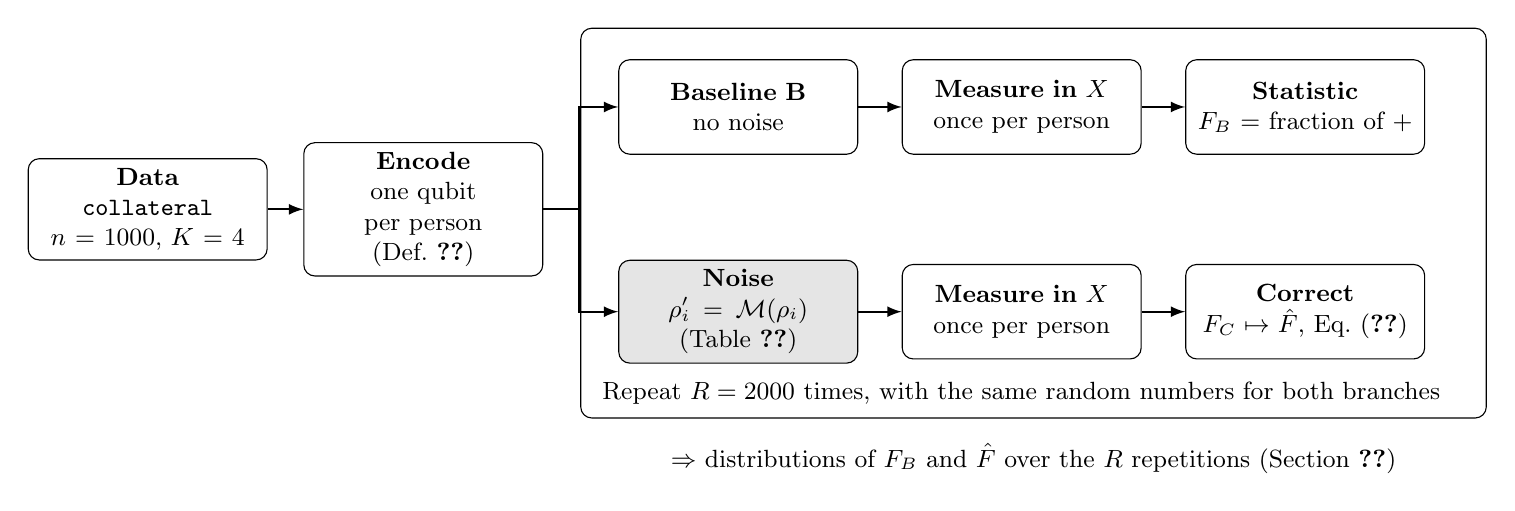
\begin{tikzpicture}[
      font=\small,
      box/.style={draw, rounded corners, align=center, text width=2.8cm, minimum height=1.2cm, fill=white},
      noisebox/.style={box, fill=gray!20},
      arr/.style={-latex, thick}
    ]
    % repetition frame (same width as Figs. 3--5)
    \draw[rounded corners] (7.4,1.0) rectangle (18.9,-3.95);
    \node[anchor=south west] at (7.55,-3.9) {Repeat $R = 2000$ times, with the same random numbers for both branches};
    % shared steps
    \node[box] (data) at (1.9,-1.3) {\textbf{Data}\\ \texttt{collateral}\\ $n = 1000$, $K = 4$};
    \node[box] (enc) at (5.4,-1.3) {\textbf{Encode}\\ one qubit per person\\ (Def.~\ref{def:encoding_categorical})};
    % branch B
    \node[box] (nb) at (9.4,0) {\textbf{Baseline B}\\ no noise};
    \node[box] (mb) at (13.0,0) {\textbf{Measure in $X$}\\ once per person};
    \node[box] (fb) at (16.6,0) {\textbf{Statistic}\\ $F_B$ = fraction of $+$};
    % branch C
    \node[noisebox] (nc) at (9.4,-2.6) {\textbf{Noise}\\ $\rho_i^{\prime} = \mathcal{M}(\rho_i)$\\ (Table~\ref{tab:shrinking_coefficient})};
    \node[box] (mc) at (13.0,-2.6) {\textbf{Measure in $X$}\\ once per person};
    \node[box] (fc) at (16.6,-2.6) {\textbf{Correct}\\ $F_C \mapsto \hat{F}$, Eq.~\eqref{eq:estimator}};
    % arrows
    \draw[arr] (data) -- (enc);
    \draw[arr] (enc.east) -- ++(0.45,0) |- (nb.west);
    \draw[arr] (enc.east) -- ++(0.45,0) |- (nc.west);
    \draw[arr] (nb) -- (mb);
    \draw[arr] (mb) -- (fb);
    \draw[arr] (nc) -- (mc);
    \draw[arr] (mc) -- (fc);
    % output
    \node[anchor=north] at (13.15,-4.15) {$\Rightarrow$ distributions of $F_B$ and $\hat{F}$ over the $R$ repetitions (Section~\ref{sec:experimental_results})};
  \end{tikzpicture}%
  }
  \caption{Experiment to measure the distributions of $F_B$ and $\hat{F}$ for $\texttt{collateral}$} 
  \label{fig:measurement_experiment}
\end{figure*}

The experiment begins by encoding the 1000 participants of the dataset into their individual qubits. Then two branches run in parallel. In branch B, each qubit is measured in the $X$ basis and we record the statistic $F_B$. In branch C, noise is applied to each qubit, resulting in the density matrix $\rho_i^{\prime} = \mathcal{M}(\rho_i)$ for the $i$-th participant, which we then measure to get $F_C$ and correct with \eqref{eq:estimator} to get $\hat{F}$; this branch is run once for each mechanism of Table~\ref{tab:shrinking_coefficient}. In both branches, each outcome is sampled with the probability given by the Born rule, $\bra{+}\rho\ket{+}$, which matches \eqref{eq:p_b} and \eqref{eq:p_c}.

Each run of the experiment represents one possible release of the data, in which every participant is measured exactly once. We call these runs repetitions rather than shots, since shots would suggest measuring the same participant many times, which is precisely what breaks the privacy guarantee. The experiment is repeated $R = 2000$ times, which gives a relative error of about $1/\sqrt{2R} \approx 1.6\%$ in the estimated standard deviations, and both branches share the same random numbers so that the noise is the only thing that changes from one branch to the other. Finally, we report the mean and standard deviation of $F_B$, $F_C$ and $\hat{F}$ over the repetitions, and compare them with \eqref{eq:expected_F_collateral}, \eqref{eq:expected_shrink} and \eqref{eq:var_fc}.

\section{Experimental Results}
\label{sec:experimental_results}

In this section we detail the results of the three experiments detailed in Sections~\ref{sec:finding_epsilon} through \ref{sec:measurement_release} in the same order that they were detailed above.

\subsection{Finding the experimental privacy budget}

\subsubsection{Central Setting}

Table~\ref{tab:central_results} compiles the results of the central setting experiment done with all three noise mechanisms. This table also includes the run with the depolarizing noise over the full $256 \times 256$ joint density matrix. On it we compiled three things: the maximum trace distance between the original matrix $\rho$ and the $j$-th leave-one-out matrix $\sigma_j$, the theoretical epsilon $\epsilon_{theo}$ and the found experimental epsilon $\epsilon_{exp}$. To help with the reader's understanding of the table all numbers were multiplied by $10^{3}$.

\begin{table*}[!t]
  \caption{Results of the $\epsilon_{theo}$ and $\epsilon_{exp}$ for the central setting experiments with all three noise mechanisms.} 
  \label{tab:central_results}
  \centering
  \begin{tabular}{clccccccc}
    \toprule
     & & \multicolumn{7}{c}{All values $\times 10^{-3}$} \\
    \cmidrule(l){3-9}
     & & & \multicolumn{2}{c}{DEP} & \multicolumn{2}{c}{PAD} & \multicolumn{2}{c}{GAD} \\
    \cmidrule(lr){4-5} \cmidrule(lr){6-7} \cmidrule(l){8-9}
    $k$ & Variable(s) & $\max_j d_j$ & $\epsilon_{theo}$ & $\epsilon_{exp}$ & $\epsilon_{theo}$ & $\epsilon_{exp}$ & $\epsilon_{theo}$ & $\epsilon_{exp}$ \\
    \midrule
    0 & \texttt{collateral}                                 & 0.567 & 1.133 & 0.608 & 1.789 & 0.758 & 2.733 & 0.887 \\
    1 & \texttt{purpose}                                    & 0.513 & 1.026 & 0.520 & 1.620 & 0.639 & 2.475 & 0.739 \\
    2 & \texttt{credit\_history}                            & 0.675 & 1.349 & 0.817 & 2.130 & 1.051 & 3.253 & 1.267 \\
    3 & \texttt{housing}                                    & 0.709 & 1.416 & 0.927 & 2.236 & 1.255 & 3.415 & 1.566 \\
    4 & \texttt{other\_installment\_plans}                  & 0.773 & 1.545 & 1.150 & 2.439 & 1.595 & 3.725 & 2.080 \\
    5 & \texttt{status\_savings}, \texttt{month\_duration}  & 0.788 & 1.574 & 1.187 & 2.486 & 1.594 & 3.796 & 2.000 \\
    6 & \texttt{years\_employment}, \texttt{credit\_amount} & 0.806 & 1.611 & 1.192 & 2.544 & 1.625 & 3.885 & 2.080 \\
    7 & \texttt{status\_account}                            & 0.708 & 1.414 & 0.943 & 2.234 & 1.020 & 3.411 & 1.100 \\
    \midrule
    \multicolumn{3}{l}{Sum over $k$ (Corollary~\ref{cor:composition})} & 11.068 & 7.345 & 17.478 & 9.537 & 26.694 & 11.721 \\
    \midrule
    \multicolumn{2}{l}{All 8 qubits, joint ($D = 256$)} & 0.999 & 227.670 & 199.849 & -- & -- & -- & -- \\
    \bottomrule
  \end{tabular}
\end{table*}

In all 24 cases, $\epsilon_{exp} < \epsilon_{theo}$. This is good as in Theorems~\ref{thm:epsilon_gad} through~\ref{thm:epsilon_dep} the $\epsilon_{theo}$ is the upper bound for epsilon. On the other hand at every iteration of Algorithm~\ref{alg:dpd} the matrices are $\rho^{\prime}$ and $\sigma^{\prime}$ rotated by a unitary $P$ (lines 6 through 8). When we calculate $\rho_{ii}$ and $\sigma_{ii}$, we are measuring over $\ket{\psi_i} = P\ket{i}$ and because $P$ is unitary, $\ket{\psi_i}$ is a unit vector. From that result, the maximum ratio $r$ of line 4 is the ratio for a particular pure state, which means that the result produced by the algorithm is at most $PD(\rho^{\prime}, \sigma_{j}^{\prime})$, since PD is no more than the supremum over all pure states (Proposition~\ref{prop:pd_pure_states}). On the other side, Theorems~\ref{thm:epsilon_gad} through~\ref{thm:epsilon_dep} guarantee that the mechanism is $\epsilon_{theo}$-differentially private (Definition~\ref{def:qdp} with $\delta = 0$) for every pair of inputs at trace distance at most $d = \max_j d_j$, which includes every leave-one-out pair $(\rho, \sigma_j)$. Taking a single outcome $S = \{m\}$ in Definition~\ref{def:qdp}, the privacy loss (Definition~\ref{def:privacy_loss}) of every outcome of every measurement is at most $\epsilon_{theo}$, and since PD is the largest of these privacy losses (Definition~\ref{def:proportional_distance}), $PD(\rho^{\prime}, \sigma_{j}^{\prime}) \leq \epsilon_{theo}$. Associating both results, we find the final bound
\begin{equation}
  \epsilon_{exp}^{j} \leq PD(\rho^{\prime}, \sigma_{j}^{\prime}) \leq \epsilon_{theo}
  \label{eq:final_bound}
\end{equation}
for every row $j$, and therefore also for $\epsilon_{exp} = \max_j \epsilon_{exp}^{j}$.

Analyzing the table some more we can see a couple more interesting results. The privacy budget computed for each mechanism holds for every column that $\epsilon_{DEP} < \epsilon_{PAD} < \epsilon_{GAD}$, this is a callback to our ``shrinking coefficient'' mentioned in Table~\ref{tab:shrinking_coefficient} and Theorems~\ref{thm:epsilon_gad} through~\ref{thm:epsilon_dep} because the $\epsilon$ increases with $s, d$ so if we hold $d$ constant then the results should align with the smallest to the biggest $s$ of Table~\ref{tab:shrinking_coefficient}. And in the case of the theo/exp ratio is $1.33 - 1.97$ for DEP, $1.53 - 2.54$ for PAD and $1.79 - 3.35$ for GAD so one could say the GAD is the loosest out of the three mechanisms.

In terms of the distance we can observe that most of them are close to $10^{-3}$ for values ranging from $0.513$ to $0.806 \times 10^{-3}$. This can be explained if we write the states we are finding the distance from $\rho$ and $\sigma_j$ as
\begin{equation}
  \rho = \frac{1}{n}\sum_{i} \rho_i, \qquad \sigma_j = \frac{1}{n-1}\sum_{i \neq j} \rho_i
  \label{eq:aggregates}
\end{equation}
but since everyone except person $j$ is just everyone minus the state of person $j$ we have
\begin{equation}
  \sum_{i \neq j} \rho_i = \sum_{i} \rho_i - \rho_j = n\rho - \rho_j
  \label{eq:sum_except_j}
\end{equation}
from \eqref{eq:aggregates} we get
\begin{equation}
  \sigma_j = \frac{n\rho - \rho_j}{n-1}
  \label{eq:sigma_j}
\end{equation}
we can rewrite \eqref{eq:sigma_j} in terms of the difference between $\rho$ and $\sigma_j$ to get
\begin{equation}
  \begin{aligned}
    n\rho &= (n-1)\sigma_j + \rho_j, \\
    \rho - \sigma_j &= \frac{\rho_j - \sigma_j}{n}
  \end{aligned}
  \label{eq:difference_neighbours}
\end{equation}
from here we can see that the difference between the two states is just the difference between the state of person $j$ and everyone else's over the number of people.

Then, calculating the distance $d_j$ with Definition~\ref{def:trace_distance}, we get
\begin{equation}
  d_j = \tau(\rho, \sigma_j) = \frac{1}{2}\Tr\abs{\rho - \sigma_j}
  \label{eq:d_j}
\end{equation}
and simplifying with \eqref{eq:difference_neighbours} we get
\begin{equation}
  \begin{aligned}
    d_j &= \frac{1}{2}\Tr\abs{\frac{\rho_j - \sigma_j}{n}} \\
        &= \frac{1}{n}\cdot\frac{1}{2}\Tr\abs{\rho_j - \sigma_j} = \frac{\tau(\rho_j, \sigma_j)}{n}
  \end{aligned}
  \label{eq:d_j_person}
\end{equation}

and considering that the largest distance between two states in the Bloch sphere is 2 (so trace distance $\tau =1$), then at most the distance can become $\frac{1}{n} = 10^{-3}$. This can also give insights as to why even though \texttt{housing} and \texttt{other\_installment\_plans} have the same $K=3$ the proportions of the categories are different and thus the relationship between a single person against the rest changes and so does the worst $d$.

Finally in Table~\ref{tab:central_results} we can observe that there is a row for the full 8 qubit side experiment. This experiment yielded a privacy budget almost 20x larger that the per qubit sum and in Section~\ref{sec:discussion_and_conclusion} we will discuss the implications this with regards to the release of the information.

\subsubsection{Local Setting}

Table~\ref{tab:local_results} shows the results of the local experiment for the variables selected. On the table we can find the number of categories $K$ each variable has, their maximum trace distance between two states, and the $\epsilon_{theo}$ and $\epsilon_{exp}$ for each variable.

\begin{table*}[!t]
  \caption{Results for the local setting experiment of finding the theoretical and experimental privacy budget $\epsilon_{theo}$ and $\epsilon_{exp}$}
  \label{tab:local_results}
  \centering
  \begin{tabular}{lcccccccc}
    \toprule
     & & & \multicolumn{2}{c}{DEP} & \multicolumn{2}{c}{PAD} & \multicolumn{2}{c}{GAD} \\
    \cmidrule(lr){4-5} \cmidrule(lr){6-7} \cmidrule(l){8-9}
    Variable & $K$ & $\max_{c,c'} d_{cc'}$ & $\epsilon_{theo}$ & $\epsilon_{exp}$ & $\epsilon_{theo}$ & $\epsilon_{exp}$ & $\epsilon_{theo}$ & $\epsilon_{exp}$ \\
    \midrule
    \texttt{collateral}                        & 4  & 1     & 1.099 & 1.099 & 1.425 & 1.425 & 1.763 & 1.763 \\
    \texttt{purpose}                           & 10 & 1     & 1.099 & 1.099 & 1.425 & 1.425 & 1.763 & 1.763 \\
    \texttt{credit\_history}                   & 5  & 0.951 & 1.065 & 1.049 & 1.388 & 1.365 & 1.721 & 1.693 \\
    \texttt{housing}                           & 3  & 0.866 & 1.005 & 0.962 & 1.318 & 1.257 & 1.645 & 1.567 \\
    \texttt{other\_installment\_plans}         & 3  & 0.866 & 1.005 & 0.962 & 1.318 & 1.257 & 1.645 & 1.567 \\
    \texttt{status\_account} (ordinal)         & 4  & 1     & 1.099 & 1.099 & 1.425 & 1.117 & 1.763 & 1.290 \\
    \bottomrule
  \end{tabular}
  \par\smallskip
  {\footnotesize For \texttt{status\_account}, the worst pair is $(0,3)$ for DEP and $(0,2)$ (or, equivalently, $(1,3)$) for PAD and GAD; for the categorical variables, every pair at the maximum distance gives the same $\epsilon$.\par}
\end{table*}

These results actually agree with the bound of Equation~\ref{eq:final_bound}. In this setting we are actually looking directly at the states that each encoding will return. For categorical variables (not ordinal) which have an even number of categories (e.g., $K=4$ or $K=10$) then we are assured that there is going to be a pair of states $c, c^{\prime}$ whose distance along the equator is going to be maximal ($d=1$) measuring the two variables along X gives the ratio found in Equation~\ref{eq:epsilon_measurement_replaced}. Which is equal for Theorems~\ref{thm:epsilon_gad} through \ref{thm:epsilon_dep} with $d=1$. For an odd number of categories (e.g., $K=3$) that bound is closer but never equal to the theoretical $\epsilon$ as the widest distance between a pair as $K$ grows will approach 1 but will never be exactly that.

Along that line these results also agree with the fact that as was mentioned in Section~\ref{subsec:experiment_local_setting} this experiment does not depend on the data. We can observe this by comparing the variables \texttt{housing} and \texttt{other\_installment\_plans} in the central and local setting. For the central setting as it was already mentioned the privacy budgets change from one variable to the other even though the number of categories remains the same because the experiment cares about each person's category relative to the others. While in the local setting the experiment only cares about the worst distance between two encoded categories, and because for \texttt{housing} and \texttt{other\_installment\_plans} there is an equal number of categories then the encoding returns the same three possible states and the worst pair is the same in both.

In the case of the ordinal variable \texttt{status\_account}, it is here that the true effects of the different encoding can be shown. The reader can recall from Section~\ref{subsec:encoding_variables} that this variable was encoded around the Y axis with a $RY$ gate, which leaves its states in the $x$--$z$ plane. Moreover, not all the mechanisms shrink the value of $x$ in the same proportion (recall Table~\ref{tab:shrinking_coefficient}) which means that, for example, for the worst pair that the experiment found, which is $120^{\circ}$ apart ($d=0.866$), the next thing that is going to matter is the shrinkage in $x$. For DEP these are the same, so the distance wins and the maximum is once again the poles. GAD and PAD agree with DEP on the poles, as there is no $x$ component between them and all three mechanisms shrink $z$ by the same factor of $0.5$, giving $\epsilon_{exp} = \ln 3$. However, since this encoding allows other pairs of categories to have an $x$ component, and GAD and PAD shrink $x$ less than $z$, a pair of categories not completely opposite to each other can give a larger $\epsilon$ ($1.290$ for GAD and $1.117$ for PAD). This is also why neither reaches its $\epsilon_{theo}$: the theorems have to cover the worst-case scenario for a given $d$, which is the pair of states that stays the furthest apart after shrinking. For GAD and PAD, this pair lies on the equator, which a variable like $\texttt{collateral}$ reaches while $\texttt{status\_account}$ does not.

One last observation that has to be mentioned is that the local $\epsilon$ is about 1000 times that of the central $\epsilon$. This might, at first glance, look like the local setting is worse overall. However, the reader might remember the explanation in Section~\ref{sec:measurement_release} about copies and what the analyst has to do to read the information of both methods, and recall that on one the $\epsilon$ is consumed $N$ times per reading while in the local setting it is consumed once. In Section~\ref{sec:discussion_and_conclusion} we will discuss this topic further.  

\subsection{Measurement and Classical release of categorical variables}
\label{subsec:measurement_results}

The last results we are going to explore are the ones for the experiment of the local measurement and release of the data. In Table~\ref{tab:measurement_results} we can observe the expected values and standard deviations of $\hat{F}$ and $F_C$ for all mechanisms, including the control, which has no noise, as well as the $\epsilon_{meas}$ and the shrinking coefficient $s$ for each one. In Figure~\ref{fig:measurement_histograms} there are three histograms which compile the distributions that $F_B$ and the corrected $\hat{F}$ had.

\begin{table*}[!t]
  \caption{Results of the measurement experiments for the statistics $F_C$ and $\hat{F}$ for the 2000 repetitions}
  \label{tab:measurement_results}
  \centering
  \begin{tabular}{lcccccccccc}
    \toprule
     & & & \multicolumn{2}{c}{$E[F_C]$} & \multicolumn{2}{c}{Std.\ dev.\ of $F_C$} & \multicolumn{2}{c}{$E[\hat{F}]$} & \multicolumn{2}{c}{Std.\ dev.\ of $\hat{F}$} \\
    \cmidrule(lr){4-5} \cmidrule(lr){6-7} \cmidrule(lr){8-9} \cmidrule(l){10-11}
    Mechanism & $s$ & $\epsilon_{meas}$ & Theo. & Sim. & Theo. & Sim. & Theo. & Sim. & Theo. & Sim. \\
    \midrule
    No noise (B: $F_B$) & --    & --    & --     & --     & --      & --      & 0.4500 & 0.4500 & 0.01044 & 0.01027 \\
    DEP                 & 0.500 & 1.099 & 0.4750 & 0.4751 & 0.01465 & 0.01426 & 0.4500 & 0.4502 & 0.02931 & 0.02852 \\
    PAD                 & 0.612 & 1.425 & 0.4694 & 0.4694 & 0.01404 & 0.01364 & 0.4500 & 0.4500 & 0.02293 & 0.02227 \\
    GAD                 & 0.707 & 1.763 & 0.4646 & 0.4646 & 0.01340 & 0.01304 & 0.4500 & 0.4500 & 0.01895 & 0.01844 \\
    \bottomrule
  \end{tabular}
\end{table*}

\begin{figure}[!t]
  \centering
  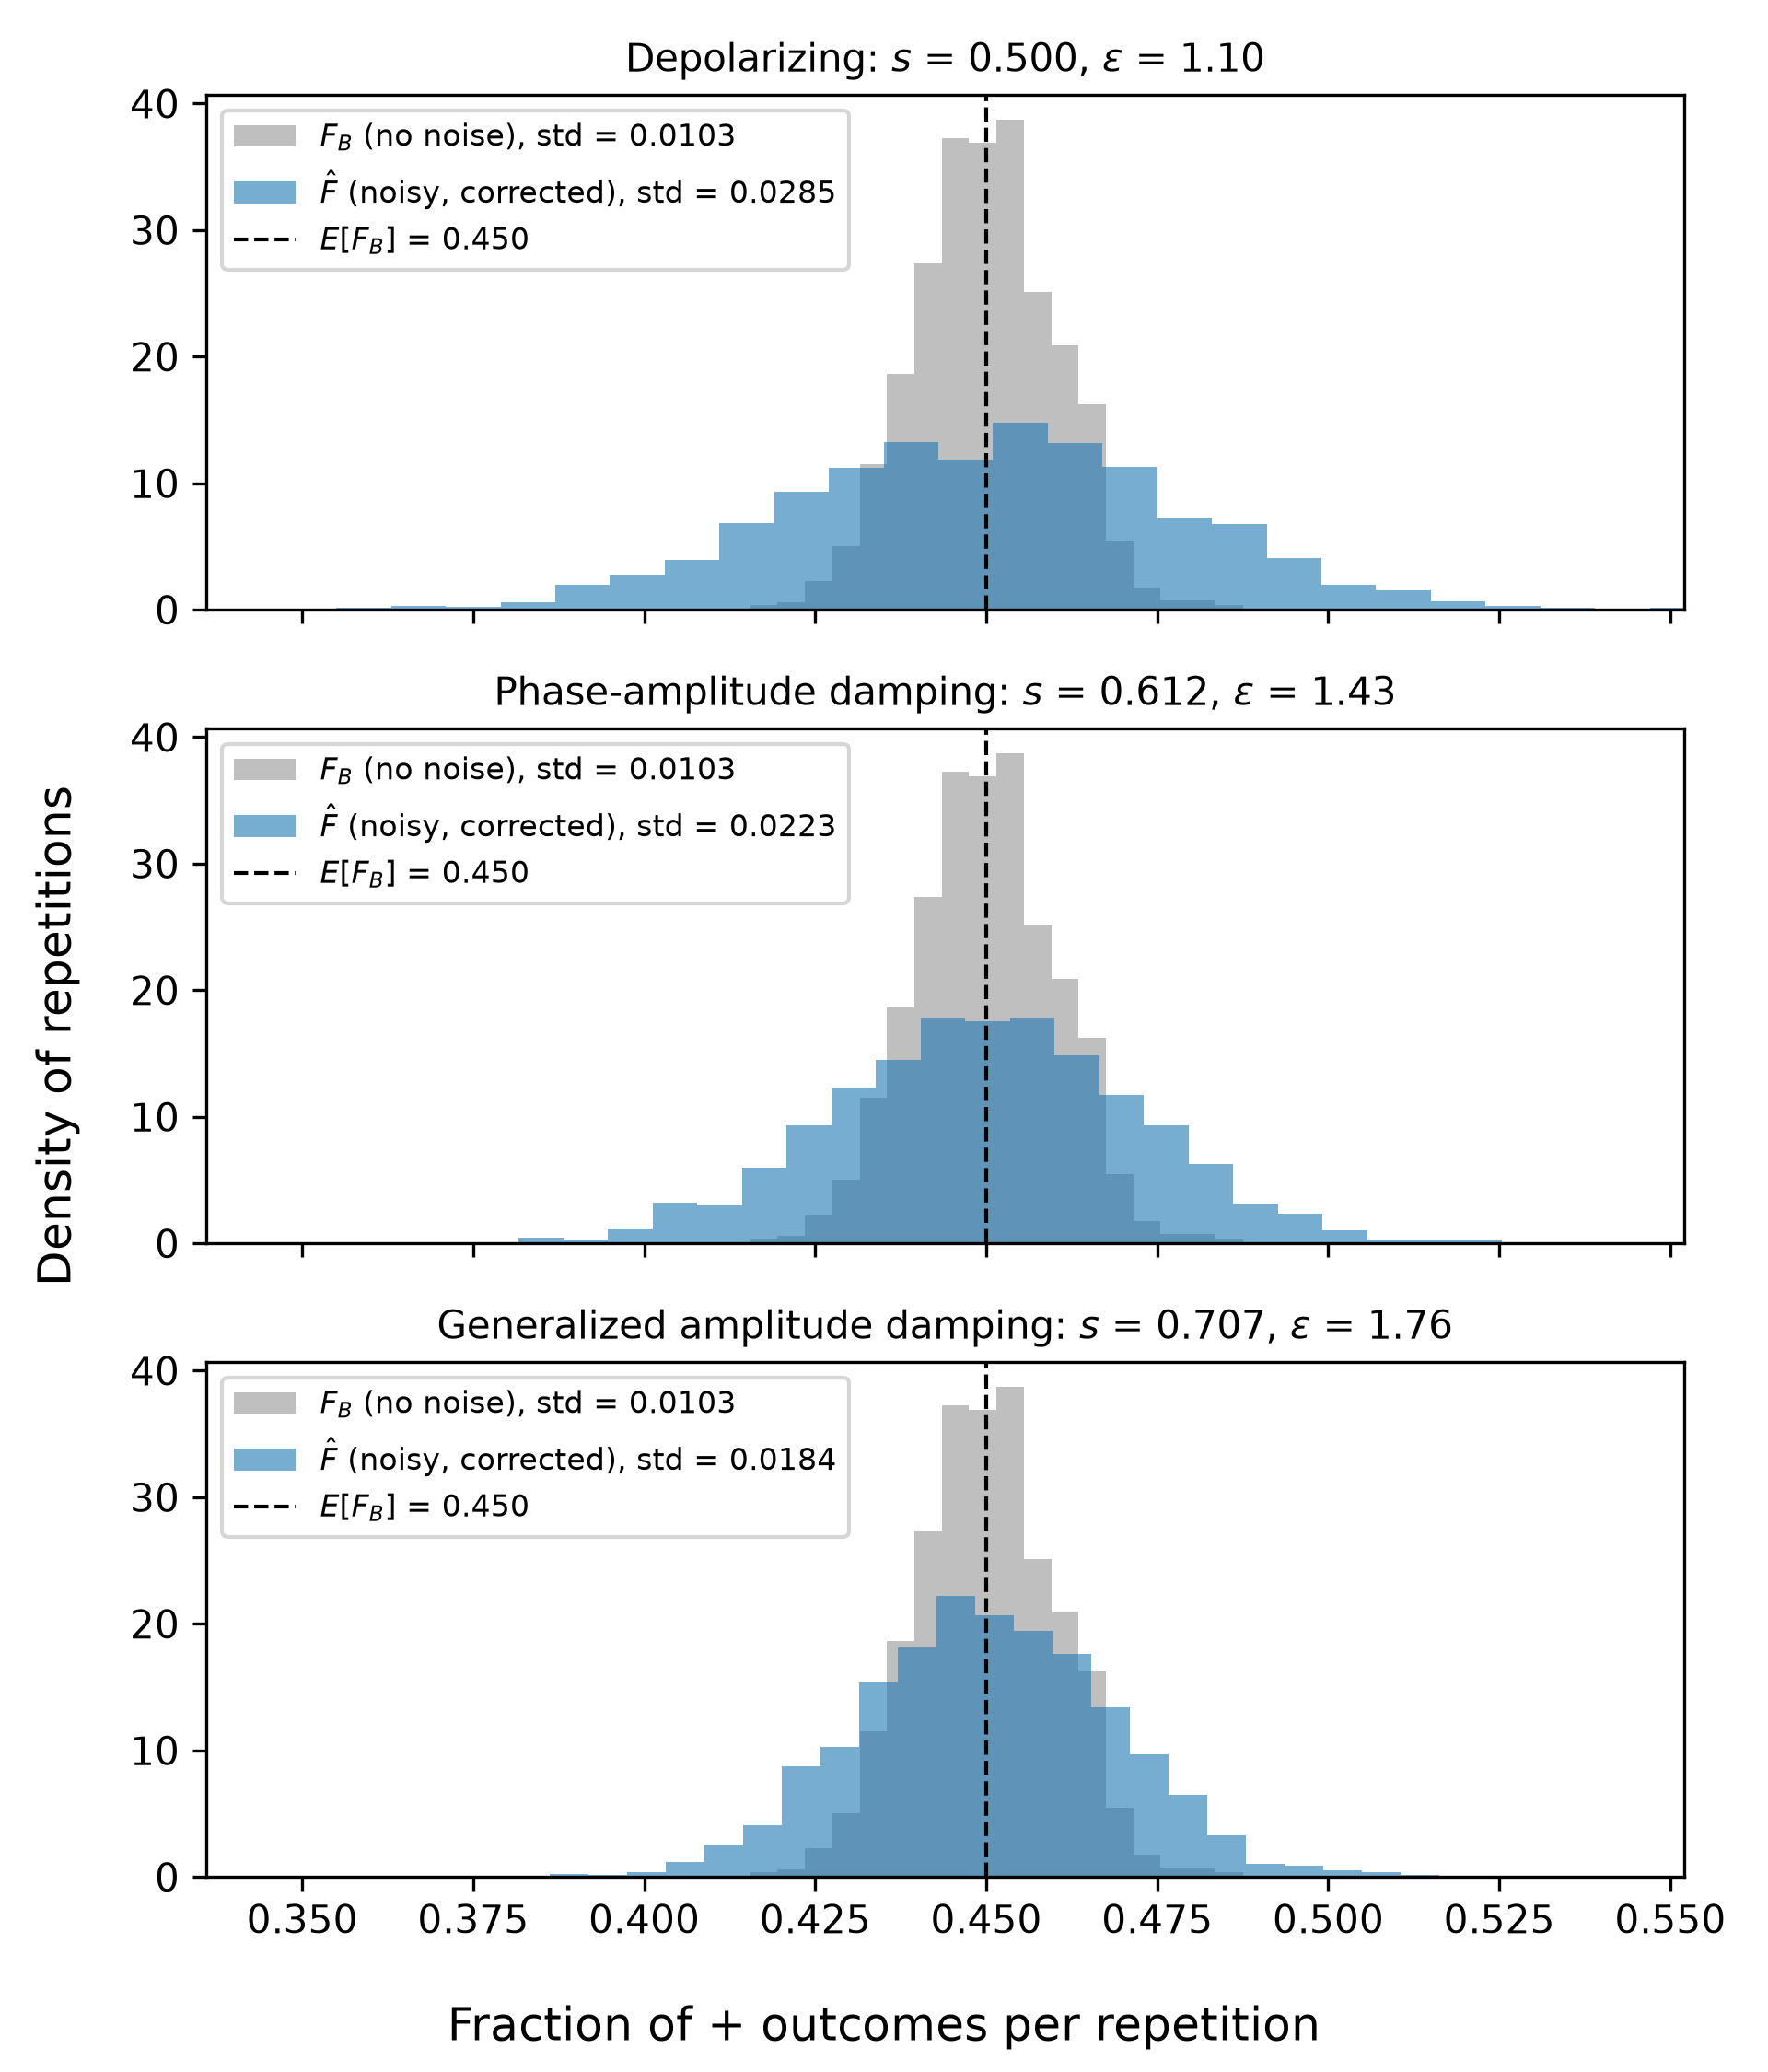
\includegraphics[width=\columnwidth]{histograma_collateral_mecanismos.png}
  \caption{Density histogram of the fraction of people whose measured state was $\ket{+}$ without noise, $F_B$, and post noise and corrected, $\hat{F}$, for DEP, PAD and GAD (top to bottom)}
  \label{fig:measurement_histograms}
\end{figure}

We can observe that the mean value of $F_C$ matches the theory and, after the correction $\hat{F}$, the mean value returns to that of $F_B$ yet the standard deviation increases in all cases. The simulated standard deviations are all slightly below the theoretical ones, by $1.6\%$ (for $F_B$) up to $2.9\%$ (for $\hat{F}$ with PAD). Since $1/\sqrt{2R} \approx 1.6\%$ is the typical size of this error (one standard error), and about $95\%$ of runs fall within two standard errors ($3.2\%$), these differences are expected. Moreover, all of them deviate in the same direction because both branches share the same random numbers, so this is a single fluctuation rather than four independent ones.

The change in the standard deviation is the real cost of privacy, which we will discuss further in Section~\ref{sec:discussion_and_conclusion}, but straight from the data of Table~\ref{tab:measurement_results} the reader can observe that each mechanism gives a standard deviation $2.78$, $2.17$ and $1.80$ times larger than $\mathrm{std}(F_B)$ in each respective case. This is thanks to Equation~\ref{eq:corrected_std}'s denominator, which results in the corrected standard deviation being inversely proportional to the shrinking coefficient and thus a smaller $s$ (more shrinking) implies a larger std. This gives a reason to the ultimate trade-off of differential privacy: with a larger $s$ (less noise), the $\epsilon$ will be bigger as people will be able to be distinguished more easily and, at the same time, the corrected $\hat{F}$ will have a more precise density.

Lastly, the reader might have noticed that the values for $\epsilon_{meas}$ are the same values that resulted from $\epsilon_{exp}$ from the local setting experiment for \texttt{collateral}. This is thanks in part to Proposition~\ref{prop:post_processing} since the measurement itself will be a quantum operation and thus be bounded by the $\epsilon$ of the noise mechanism. Moreover, the variable \texttt{collateral} measured with $X$ will give complete distinction between the worst pair without noise (car and real estate). After noise, as shown in Equation~\ref{eq:epsilon_measurement_replaced}, the value will be reached for the states which result in the longest trace distance $d=1$ apart.


\section{Discussion and Conclusion}
\label{sec:discussion_and_conclusion}


The first contribution of this investigation was a framework to encode classical data into quantum states, which was later used in our proposed experiments to study the effects of differential privacy in quantum simulations.

In the central setting experiment we found how loose $\epsilon_{theo}$ is with respect to the experimental result $\epsilon_{exp}$. As shown in Equation~\eqref{eq:final_bound}, $\epsilon_{exp}$ is a lower bound for the true privacy budget, and thus the actual budget of the dataset lies in $[\epsilon_{exp}, \epsilon_{theo}]$. Since our estimate never reached this upper bound, a curator who sets the privacy budget to $\epsilon_{theo}$ has an assurance of privacy, but may be trading usefulness for privacy that the dataset does not need. The curator cannot use $\epsilon_{exp}$ instead, since it is only a lower bound.

In the local setting, where each data subject is responsible for adding noise to their own data, the privacy budget is much bigger (about 1000 times that of the central setting). At first glance this might look like a straight argument to only use the central setting when protecting data; however, as seen in Section~\ref{sec:measurement_release}, this comes with a trade-off. Because of the no-cloning theorem, the analyst needs $N$ independent copies to read the central state, so the smaller $\epsilon$ is spent $N$ times, resulting in a total privacy budget of $N\epsilon$ (Corollary~\ref{cor:composition}). On the other hand, the bigger budget of the local mechanism is spent only once, as each person measures their own state a single time. For the single qubit of \texttt{collateral} under DEP and $N = 1000$ copies (the same number of outcomes the local release gets, one per person), neither method is clearly better: in the central setting $\epsilon_{tot} = 1000 \times 0.000608 = 0.608$, while in the local setting $\epsilon = 1.099$.

Lastly, one might try to apply the noise directly on the full 8-qubit density matrix, as the DEP mechanism allows. However, the resulting $\epsilon$ is about 20 to 27 times bigger than the sum of the per-qubit budgets. This is because in Theorem~\ref{thm:epsilon_dep} $\epsilon$ grows with $D$: in Definition~\ref{def:dep}, a bigger $D$ spreads the identity term over more dimensions, so each direction receives only $p/D$ of the noise, while $\rho$ is still only compressed by a factor of $(1-p)$. Since this is also a central release, the same reasoning about measurement applies, and with $N = 1000$ copies the total budget becomes $\epsilon_{tot} = 1000 \times 0.199849 = 199.849$, which makes this method completely useless to protect the data.

This investigation also provided an approach to understand the true cost of privacy. As seen in Subsection~\ref{subsec:measurement_results}, after the noise and the correction the standard deviation of $\hat{F}$ increases, which means that the released values become more dispersed around the original mean. Both effects come from the same shrinking coefficient $s$: a smaller $s$ lowers $\epsilon_{meas}$, so an attacker has less chance of identifying a single person, but it also widens the standard deviation, so the analyst gets a less precise estimate.

This investigation has two main limitations. First, the experiments were carried out on quantum simulators, where the noise channels are applied exactly through their Kraus operators. On real hardware these operations are more difficult to carry out, since they require extra environment qubits to produce the decoherence and measurement shots to estimate the resulting states. Second, the proposed encoding and the experiments to measure the privacy budget respond to specific choices: the German Credit dataset and a single set of noise parameters (Table~\ref{tab:noise_params}).

All in all, the investigation achieved its objective, which was to compare and contrast the theoretical privacy budget $\epsilon$ of different quantum noise mechanisms with an experimental one in quantum computing simulations. Each experiment yielded results that align with the expectations founded on~\cite{zhou2017differential} and~\cite{dwork2014algorithmic}, among many other works studied to bring this investigation to fruition. As future work we propose implementing the mechanisms on real hardware, parameter sweeps, a comparison with the Lifted QDP of Song et al.~\cite{song2025hybrid}, and joining this investigation with variational quantum circuits to build a private quantum machine learning pipeline.

\clearpage
\appendices

\renewcommand{\thelemma}{\Alph{section}.\arabic{lemma}}
\renewcommand{\theproposition}{\Alph{section}.\arabic{proposition}}

\section{Description of selected features}
\label{ap:selected_features}

Table~\ref{tab:variables_descriptions} compiles the name, type and description of the variables that were selected for use in the quantum experiments.

\begin{table*}[!t]
  \caption{Description of the selected variables.}
  \label{tab:variables_descriptions}
  \centering
  \begin{tabular}{llp{0.5\textwidth}}
    \toprule
    Name & Type & Description \\
    \midrule
    \texttt{status\_account}           & Categorical (Ordinal)     & Status of the existing checking account, in DM (Deutsche Marks) \\
    \texttt{month\_duration}           & Numerical   & Duration of the credit in months \\
    \texttt{credit\_amount}            & Numerical   & Credit amount \\
    \texttt{collateral}                & Categorical & Possible collateral for the loan \\
    \texttt{purpose}                   & Categorical & Purpose of the credit \\
    \texttt{credit\_history}           & Categorical & Credit history of the applicant \\
    \texttt{housing}                   & Categorical & Current housing situation (rented, owned, or free) \\
    \texttt{years\_employment}         & Categorical (Ordinal)     & Length of time in current employment \\
    \texttt{status\_savings}           & Categorical (Ordinal)     & Status of the savings account, in DM (Deutsche Marks) \\
    \texttt{other\_installment\_plans} & Categorical & Whether the client has other installment plans \\
    \bottomrule
  \end{tabular}
\end{table*}

\section{Description of label assigned to each categorical variable}
\label{ap:label_categorical}

Table~\ref{tab:label_categorical} compiles the labels given to each variable's categories using the scikit-learn Python library.

\begin{table*}[!t]
  \caption{Assignment of the label given to each categorical variable's category}
  \label{tab:label_categorical}
  \centering
  \begin{tabular}{llc}
    \toprule
    Variable & Category & Label \\
    \midrule
    \multirow{4}{*}{\texttt{collateral}}
      & car & 0 \\
      & none & 1 \\
      & real estate & 2 \\
      & savings agreement/life insurance & 3 \\
    \midrule
    \multirow{10}{*}{\texttt{purpose}}
      & business & 0 \\
      & car (new) & 1 \\
      & car (used) & 2 \\
      & domestic appliances & 3 \\
      & education & 4 \\
      & furniture/equipment & 5 \\
      & others & 6 \\
      & radio/television & 7 \\
      & repairs & 8 \\
      & retraining & 9 \\
    \midrule
    \multirow{5}{*}{\texttt{credit\_history}}
      & all credits at this bank paid back duly & 0 \\
      & critical account/ other credits existing (not at this bank) & 1 \\
      & delay in paying off in the past & 2 \\
      & existing credits paid back duly till now & 3 \\
      & no credits taken/ all credits paid back duly & 4 \\
    \midrule
    \multirow{3}{*}{\texttt{housing}}
      & for free & 0 \\
      & own & 1 \\
      & rent & 2 \\
    \midrule
    \multirow{3}{*}{\texttt{other\_installment\_plans}}
      & bank & 0 \\
      & none & 1 \\
      & stores & 2 \\
    \bottomrule
  \end{tabular}
\end{table*}

\section{$\phi_{K}$ correlation for all combinations of numerical and ordinal variables}
\label{ap:phik_numerical_ordinal}

Table~\ref{tab:phik_numerical_ordinal} shows the $\phi_{K}$ correlation results for all combinations of numerical and ordinal variables, as well as their worst correlation between the two pairs.

\begin{table*}[htbp]
  \caption{Comparison of variable pairs and PhiK metrics}
  \label{tab:phik_numerical_ordinal}
  \centering
  \setlength{\tabcolsep}{4pt}
  \begin{tabular}{@{}lllrrr@{}}
  \toprule
   & & & \multicolumn{3}{c}{$\phi_K$} \\
  \cmidrule(l){4-6}
  Alone & First pair & Second pair & First pair & Second pair & Worst \\
  \midrule
  \texttt{status\_account} & \texttt{status\_savings}, \texttt{month\_duration} & \texttt{years\_employment}, \texttt{credit\_amount} & 0.000 & 0.043 & 0.043 \\
  \texttt{credit\_amount} & \texttt{status\_account}, \texttt{years\_employment} & \texttt{status\_savings}, \texttt{month\_duration} & 0.088 & 0.000 & 0.088 \\
  \texttt{status\_savings} & \texttt{status\_account}, \texttt{month\_duration} & \texttt{years\_employment}, \texttt{credit\_amount} & 0.091 & 0.043 & 0.091 \\
  \texttt{status\_account} & \texttt{status\_savings}, \texttt{credit\_amount} & \texttt{years\_employment}, \texttt{month\_duration} & 0.092 & 0.065 & 0.092 \\
  \texttt{years\_employment} & \texttt{status\_account}, \texttt{month\_duration} & \texttt{status\_savings}, \texttt{credit\_amount} & 0.091 & 0.092 & 0.092 \\
  \texttt{month\_duration} & \texttt{status\_account}, \texttt{years\_employment} & \texttt{status\_savings}, \texttt{credit\_amount} & 0.088 & 0.092 & 0.092 \\
  \texttt{status\_savings} & \texttt{status\_account}, \texttt{credit\_amount} & \texttt{years\_employment}, \texttt{month\_duration} & 0.114 & 0.065 & 0.114 \\
  \texttt{years\_employment} & \texttt{status\_account}, \texttt{credit\_amount} & \texttt{status\_savings}, \texttt{month\_duration} & 0.114 & 0.000 & 0.114 \\
  \texttt{credit\_amount} & \texttt{status\_account}, \texttt{month\_duration} & \texttt{status\_savings}, \texttt{years\_employment} & 0.091 & 0.150 & 0.150 \\
  \texttt{month\_duration} & \texttt{status\_account}, \texttt{credit\_amount} & \texttt{status\_savings}, \texttt{years\_employment} & 0.114 & 0.150 & 0.150 \\
  \texttt{credit\_amount} & \texttt{status\_account}, \texttt{status\_savings} & \texttt{years\_employment}, \texttt{month\_duration} & 0.200 & 0.065 & 0.200 \\
  \texttt{month\_duration} & \texttt{status\_account}, \texttt{status\_savings} & \texttt{years\_employment}, \texttt{credit\_amount} & 0.200 & 0.043 & 0.200 \\
  \texttt{status\_account} & \texttt{status\_savings}, \texttt{years\_employment} & \texttt{credit\_amount}, \texttt{month\_duration} & 0.150 & 0.689 & 0.689 \\
  \texttt{status\_savings} & \texttt{status\_account}, \texttt{years\_employment} & \texttt{credit\_amount}, \texttt{month\_duration} & 0.088 & 0.689 & 0.689 \\
  \texttt{years\_employment} & \texttt{status\_account}, \texttt{status\_savings} & \texttt{credit\_amount}, \texttt{month\_duration} & 0.200 & 0.689 & 0.689 \\
  \bottomrule
  \end{tabular}
\end{table*}

\section{Per-qubit noise as a combined mechanism}
\label{ap:composition_proof}

In this appendix we prove Lemma~\ref{lem:product_channel} which is used in Section~\ref{sec:finding_epsilon} in order to allow for the addition of the $\epsilon_{theo}^{k}$ and $\epsilon_{exp}^{k}$ for the $k$ qubits by demonstrating that the tensor product of the outputs, $\bigotimes_i\mathcal{E}_i(\rho_i)$, is the same as the tensor product of the operations applied to the tensor product of the states, $(\bigotimes_{i}\mathcal{E}_i)(\bigotimes_{i}\rho_i)$.

\begin{lemma}
  Let $X_i$ and $U_i$ be linear operators on a vector space $\mathcal{H}_i$, for $i = 1, \dots, k$. Then
  \[
    \Big(\bigotimes_{i=1}^{k} X_i\Big)\Big(\bigotimes_{i=1}^{k} U_i\Big) = \bigotimes_{i=1}^{k} X_i U_i.
  \]
  \label{lem:mixed_product}
\end{lemma}

\begin{IEEEproof}
  Two linear operators are equal if and only if they act in the same way on every vector of the space. The product vectors $e_1 \otimes \dots \otimes e_k$, with each $e_i$ taken from a basis of $\mathcal{H}_i$, span $\bigotimes_{i} \mathcal{H}_i$, and both sides are linear, so it is enough to compare them on these vectors. By the definition of the tensor product of operators, $(\bigotimes_i T_i)(\bigotimes_i v_i) = \bigotimes_i T_i v_i$~\cite[Eq.~(1.8)]{zwiebach2013tensor}.
  Therefore
  \begin{align*}
    \Big(\bigotimes_{i} X_i\Big)\Big(\bigotimes_{i} U_i\Big)\Big(\bigotimes_{i} e_i\Big)
      &= \Big(\bigotimes_{i} X_i\Big)\Big(\bigotimes_{i} U_i e_i\Big) \\
      &= \bigotimes_{i} X_i U_i e_i \\
      &= \Big(\bigotimes_{i} X_i U_i\Big)\Big(\bigotimes_{i} e_i\Big),
  \end{align*}
  so both operators agree on every product vector, and hence on all of $\bigotimes_i \mathcal{H}_i$.
\end{IEEEproof}

\begin{proposition}
  Let $A_i$ be a linear operator and $\rho_i$ a density operator on $\mathcal{H}_i$, for $i = 1, \dots, k$. Then
  \begin{align*}
    \Big(\bigotimes_{i=1}^{k} A_i\Big)\Big(\bigotimes_{i=1}^{k} \rho_i\Big)&\Big(\bigotimes_{i=1}^{k} A_i\Big)^{\dagger} \\
      &= \bigotimes_{i=1}^{k} A_i \rho_i A_i^{\dagger}.
  \end{align*}
  \label{prop:product_operation}
\end{proposition}

\begin{IEEEproof}
  The adjoint of a tensor product is the tensor product of the adjoints, $(\bigotimes_i A_i)^{\dagger} = \bigotimes_i A_i^{\dagger}$~\cite{Nielsen_Chuang_2010}. % TODO: add the section number once read
  Applying Lemma~\ref{lem:mixed_product} twice,
  \begin{align*}
    \Big(\bigotimes_{i} A_i\Big)\Big(\bigotimes_{i} \rho_i\Big)\Big(\bigotimes_{i} A_i^{\dagger}\Big)
      &= \Big(\bigotimes_{i} A_i\Big)\Big(\bigotimes_{i} \rho_i A_i^{\dagger}\Big) \\
      &= \bigotimes_{i} A_i \rho_i A_i^{\dagger}.
  \end{align*}
\end{IEEEproof}

\begin{IEEEproof}[Proof of Lemma~\ref{lem:product_channel}]
  The operation $\bigotimes_i \mathcal{E}_i$ has Kraus operators $E_{1,a_1} \otimes \dots \otimes E_{k,a_k}$, one for each choice of indices $a_1, \dots, a_k$. Applying Proposition~\ref{prop:product_operation} to each term, and then the distributivity (bilinearity) of the tensor product over sums,
  \begin{align*}
    &\Big(\bigotimes_{i} \mathcal{E}_i\Big)\Big(\bigotimes_{i} \rho_i\Big) \\
    &\quad= \sum_{a_1, \dots, a_k} \Big(\bigotimes_{i} E_{i,a_i}\Big)\Big(\bigotimes_{i} \rho_i\Big)\Big(\bigotimes_{i} E_{i,a_i}\Big)^{\dagger} \\
    &\quad= \sum_{a_1, \dots, a_k} \bigotimes_{i} E_{i,a_i}\, \rho_i\, E_{i,a_i}^{\dagger} \\
    &\quad= \bigotimes_{i} \sum_{a_i} E_{i,a_i}\, \rho_i\, E_{i,a_i}^{\dagger}
       = \bigotimes_{i} \mathcal{E}_i(\rho_i).
  \end{align*}
\end{IEEEproof}

\clearpage
\raggedbottom
\section*{Acknowledgments}
\label{sec:acknowledgment}

Esta seccion solo para la tesis o no se si pueda ir en el paper tambien

\bibliographystyle{IEEEtran}
\bibliography{references}


\EOD 

\end{document}
